\chapter{Feature Engineering and Feature Selection \label{chapter:featureengineering}}

The methods we've studied in Chapters~\ref{chapter:classification} and \ref{chapter:regression}, as well as all other supervised (and unsupervised) machine learning algorithms, all depend on the concept of a \textbf{feature}. A feature is some aspect of each training example that the model designer believes will influence its relationship to the outcome, or that captures some aspect of the data in a way that is relevant to the problem he/she is trying to solve. 

Before any algorithm can be applied, therefore, it is necessary to decide how to represent the data: which features to include and how to extract them from the raw data. This task is called \textbf{feature engineering}. In most cases, the model designer will also want to incorporate some form of \textbf{feature selection}: a process that automatically or semi-automatically decides which features are most relevant to the model and discards the others.

\vspace{5mm}

\begin{question}{}
Choose 2-3 examples from the list of problems in Section~\ref{section:projectexamples}. Describe the setup of each problem and what types of features one would need to collect to build an accurate/useful model. 
\end{question}

%%%%%%%%%%%%%%%%%%%%%%%%%%%%%%%%%%%%%%%%%%%%%%%%%%%%%%%%%%%%%%%%%%%%%%

\section{Sample Dataset}

The so-called ``Pima Indians diabetes dataset'' was collected in the 1980s. It includes information on 768 women from the Pima people, who live near Phoenix, Arizona. The Pima were, as of the late 1980s, under continuous study by the National Institute of Diabetes and Digestive and Kidney Diseases because of their high incidence of diabetes\footnote{The causative factors behind this high diabetes rate are not clear. Some scholars believe that it was driven by a sudden shift in diet during the last century from traditional agricultural crops to processed foods, together with a decline in physical activity \cite{schulz2006effects}.}. There are eight predictors in the dataset and one outcome. The predictors are:
\begin{center}
\texttt{ \small
\begin{tabular}{lp{0.6\textwidth}}
\toprule
Predictor & Description \\
\midrule
Pregnancies & Number of times pregnant \\
Glucose & Plasma glucose concentration in a two-hour oral glucose tolerance test \\
BloodPressure & Diastolic blood pressure (mm Hg) \\
SkinThickness & Triceps skin fold thickness (mm) \\
Insulin & Two-hour serum insulin ($\mu$U/mL) \\
BMI & Body mass index (weight in kg/(height in m)$^2$) \\
DiabetesPedigreeFunction & Diabetes pedigree function (developed by research team; described in paper) \\
Age & Age in years \\
\bottomrule
\end{tabular}
}
\end{center}

The outcome is whether or not the woman went on to develop type II diabetes within $5$~years from the time of the survey. 

\begin{question}{}
Why is coding this outcome as 0/1, or yes/no, potentially problematic?
\end{question}

\begin{question}{}
What type of problem is this? What methods should we consider when solving this problem? Name at least three learning algorithms that might be appropriate. 
\end{question}

%%%%%%%%%%%%%%%%%%%%%%%%%%%%%%%%%%%%%%%%%%%%%%%%%%%%%%%%%%%%%%%%%%%%%%

\section{Feature Engineering}

Feature engineering mostly depends on domain expertise. There are three major analytical considerations when performing feature engineering: how the raw data is represented/summarized into features, how those features enter the model (e.g., do they need to be transformed or combined), and how different features are related to each other. 

\subsection{Representation}

Rarely will raw data, especially observational data, feed directly into a model. More often, one must decide how to design features that capture aspects of the data that are likely to be important to the model. 

\vspace{2mm}

\begin{question}{}
These histograms show the distributions of the individual predictors in the Pima dataset. In each case, what is one alternative way that the same information could be represented as a feature? For predictors 2--6, what do you think the zero values mean and how should they be dealt with?
  \begin{enumerate}
  \item Pregnancies
    \begin{center}
    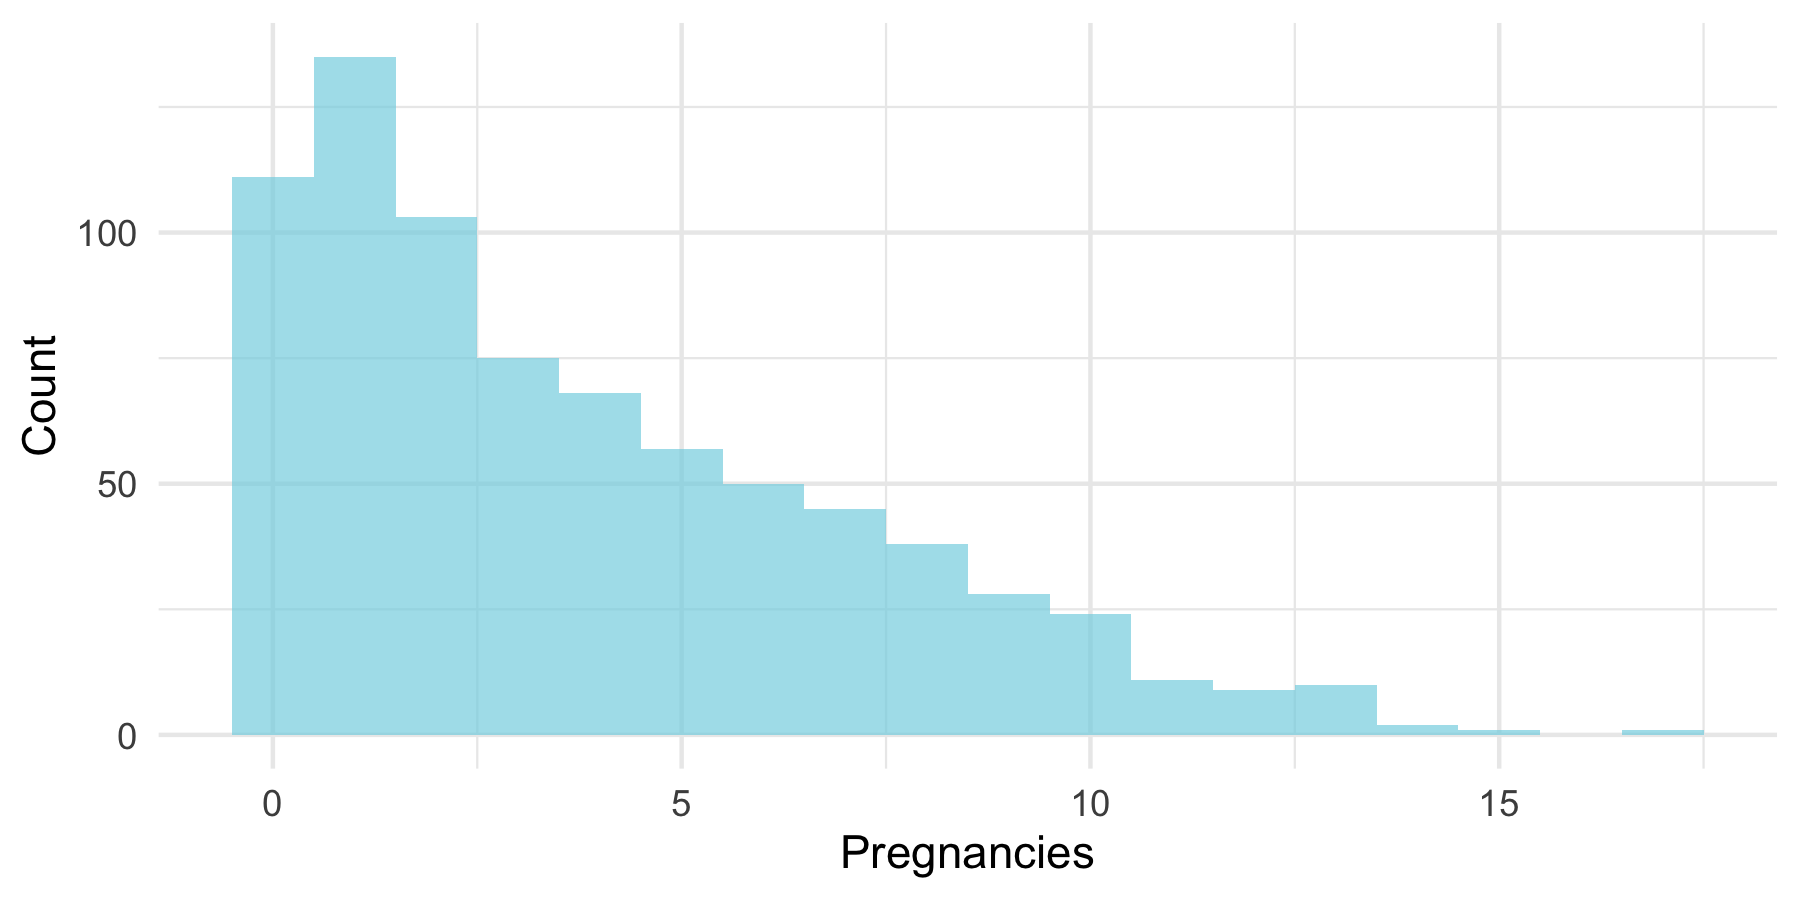
\includegraphics[width=0.65\textwidth]{img/pima-pregnancies.png}
    \end{center}
    \newpage
  \item Glucose
    \begin{center}
    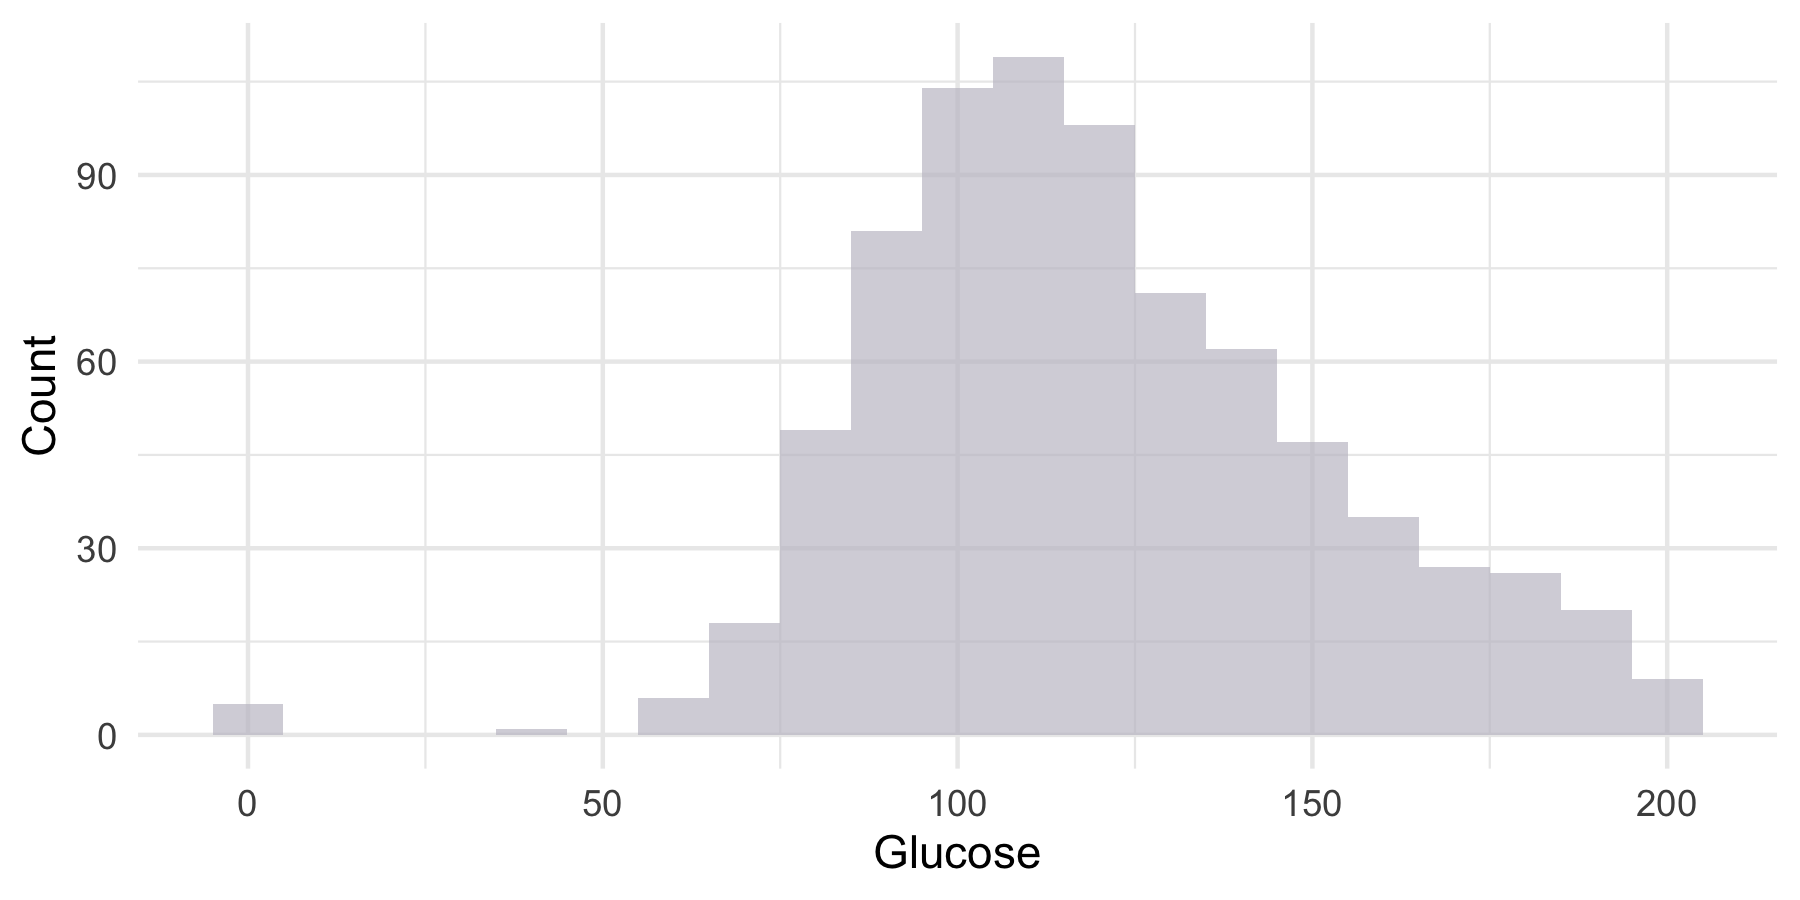
\includegraphics[width=0.65\textwidth]{img/pima-glucose.png}
    \end{center}
  \item BloodPressure
    \begin{center}
    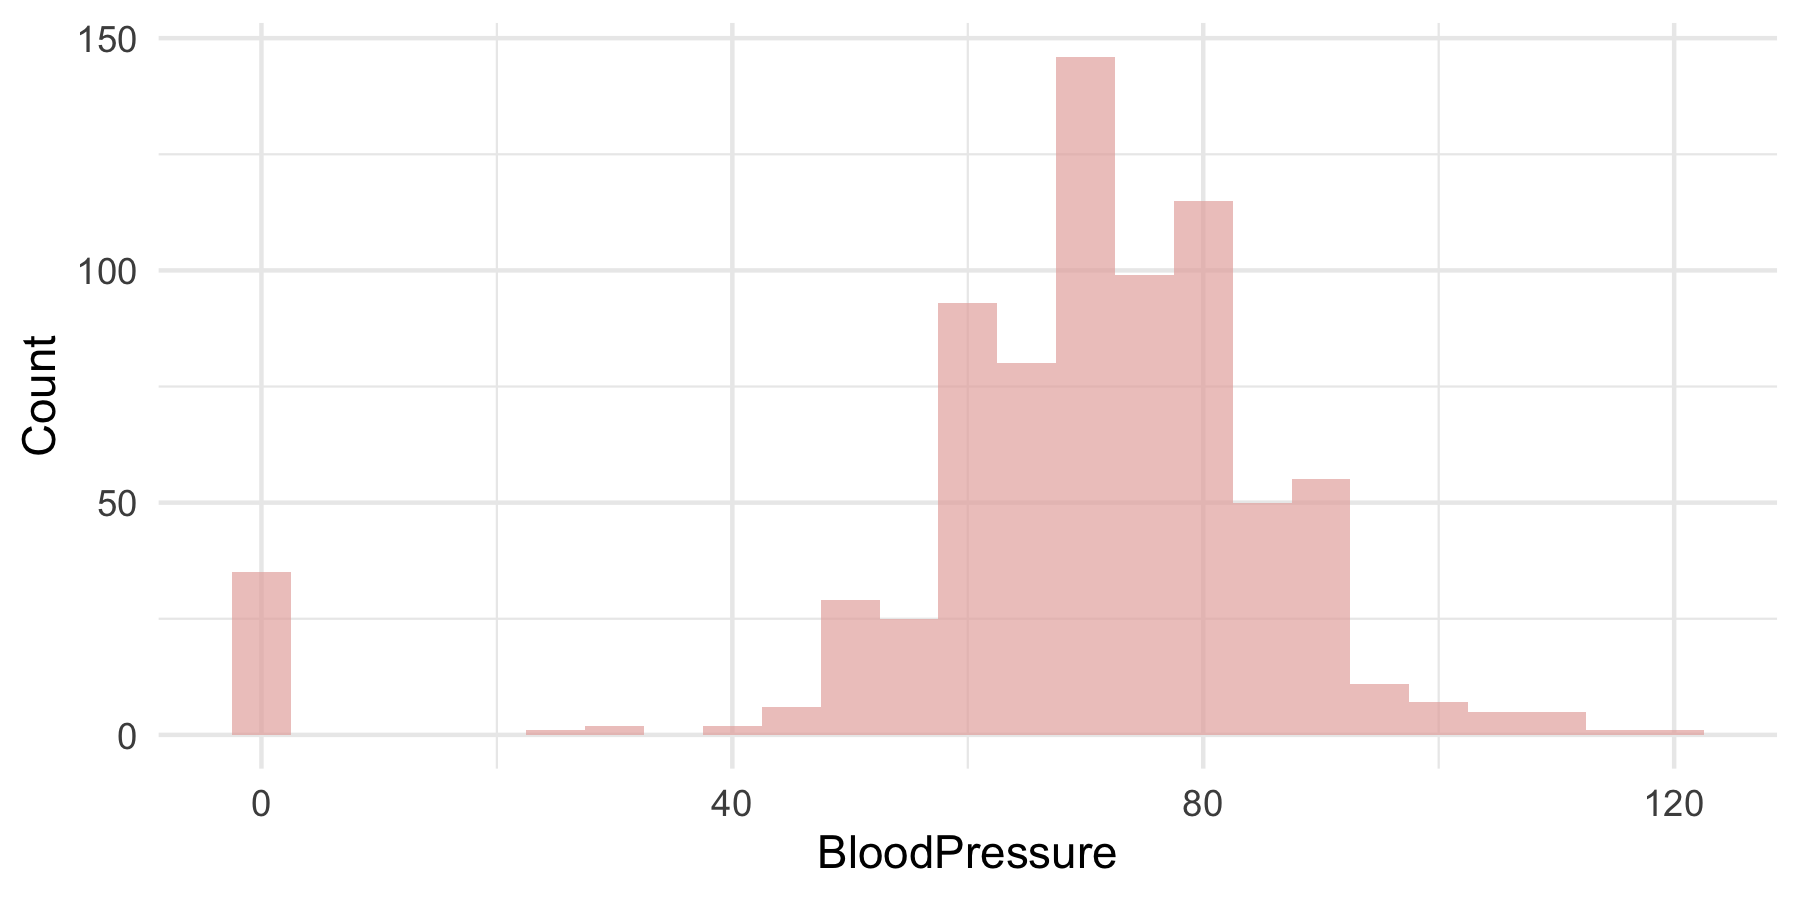
\includegraphics[width=0.65\textwidth]{img/pima-blood-pressure.png}
    \end{center}
  \item SkinThickness
    \begin{center}
    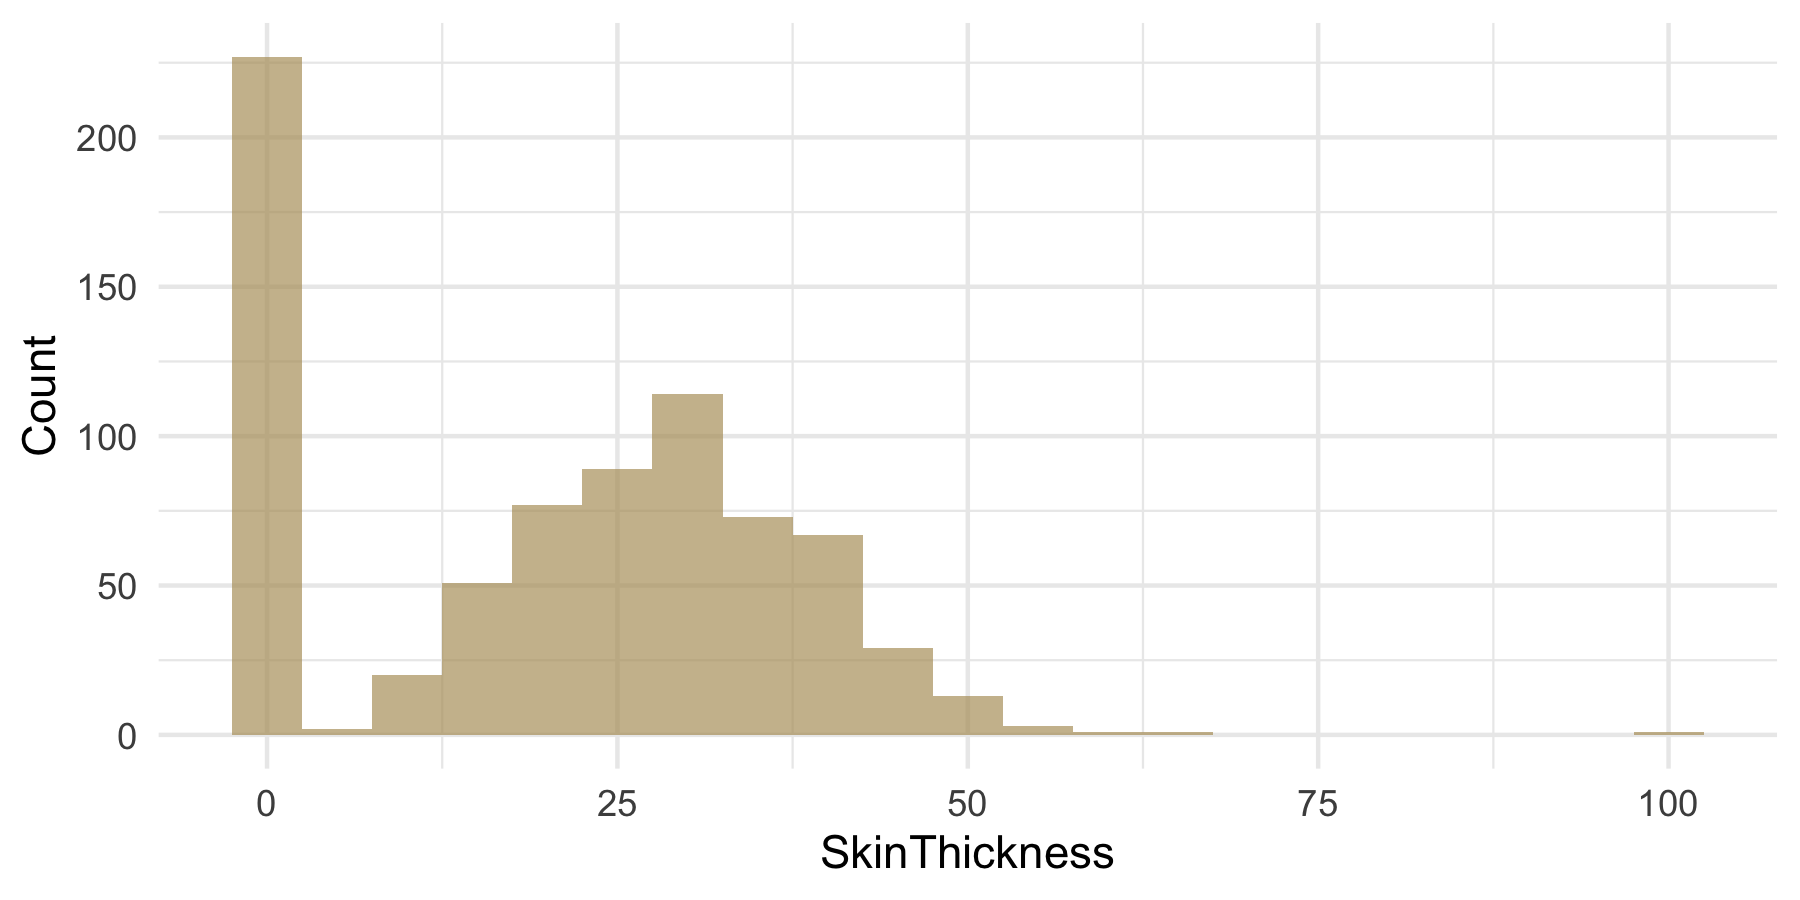
\includegraphics[width=0.65\textwidth]{img/pima-skin-thickness.png}
    \end{center}
    \newpage
  \item Insulin
    \begin{center}
    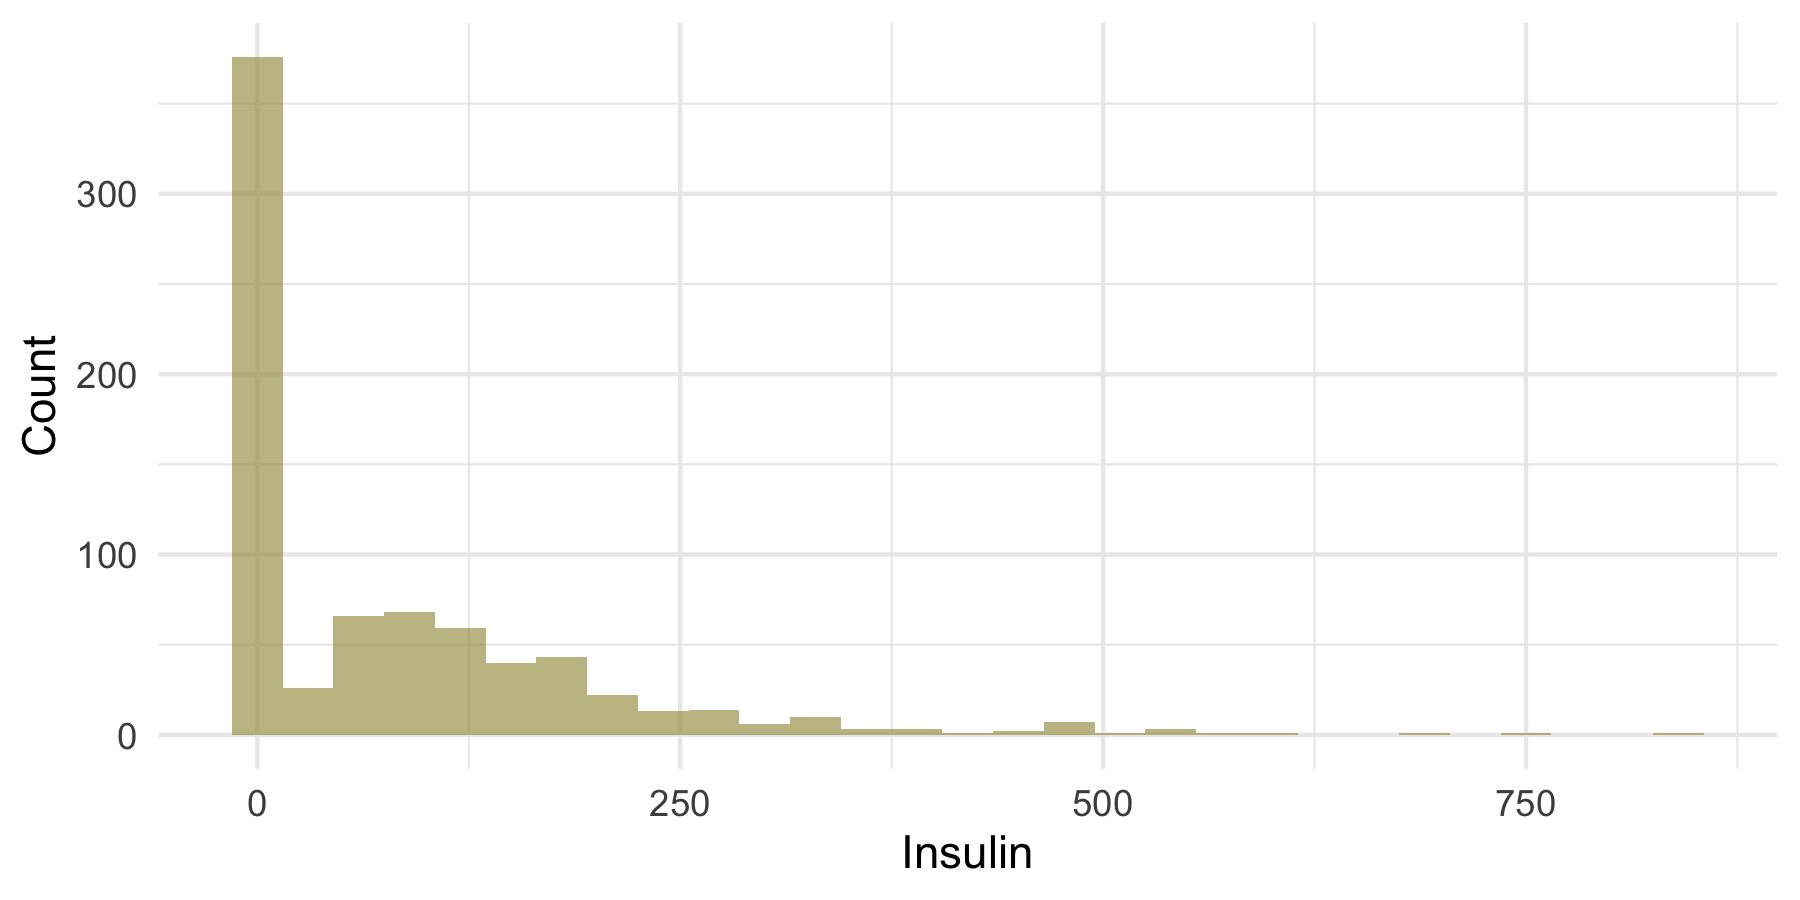
\includegraphics[width=0.65\textwidth]{img/pima-insulin.png}
    \end{center}
  \item BMI
    \begin{center}
    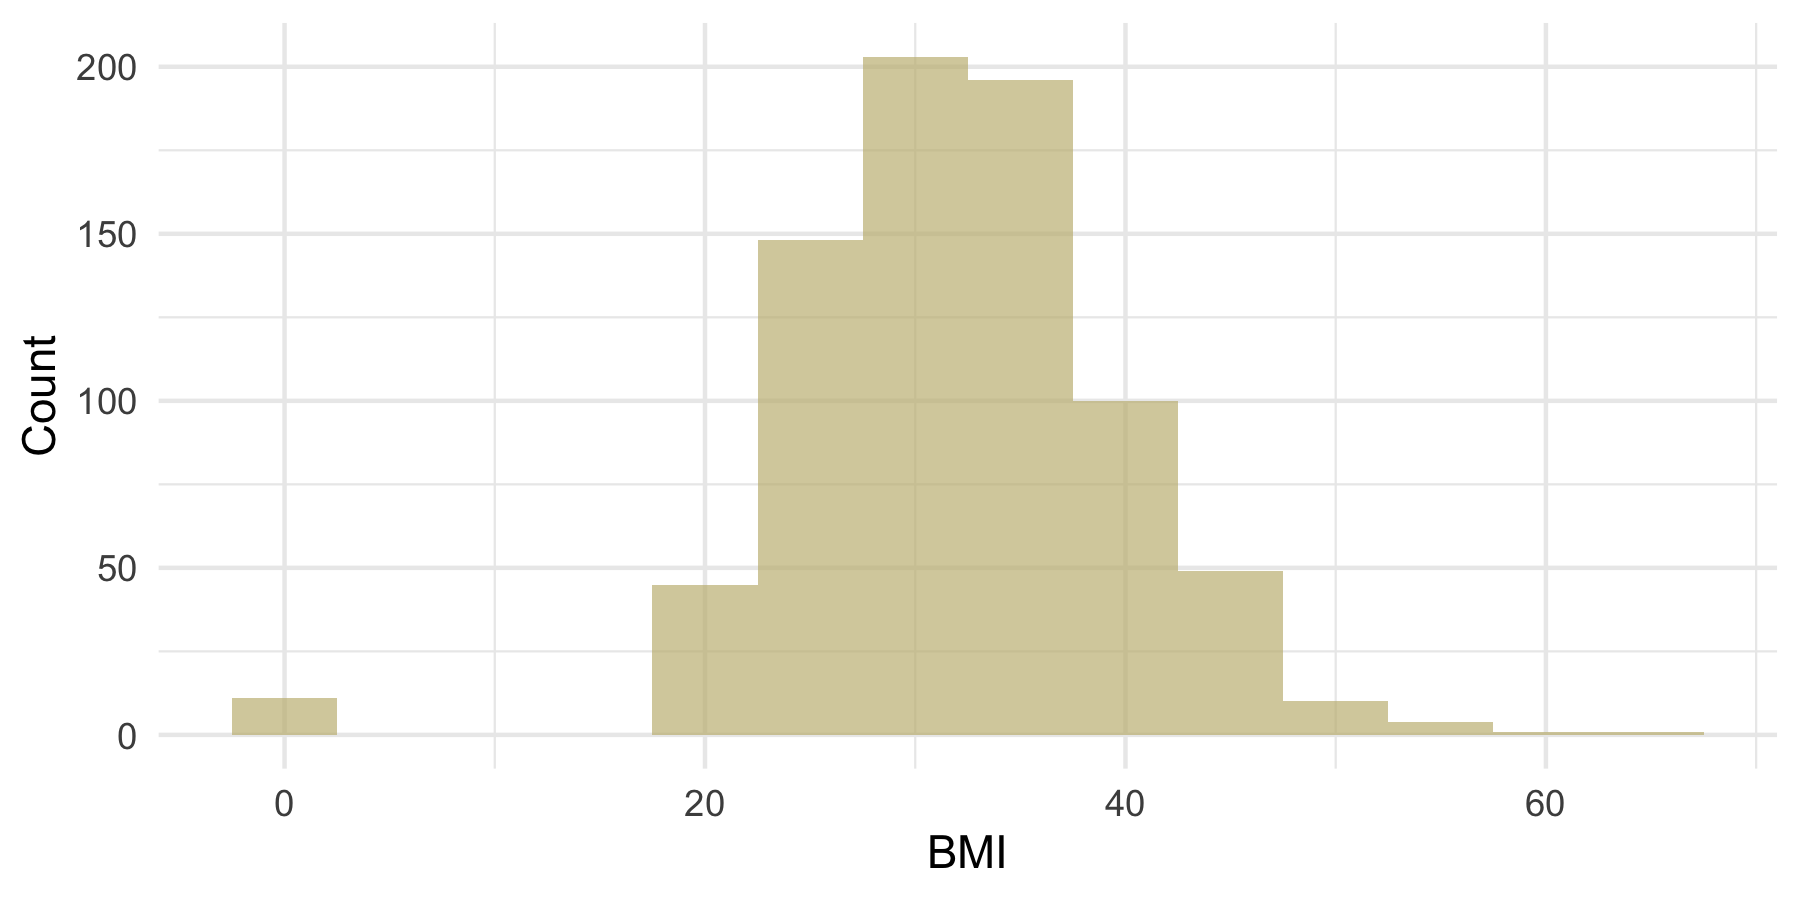
\includegraphics[width=0.65\textwidth]{img/pima-bmi.png}
    \end{center}
  \item DiabetesPedigreeFunction
    \begin{center}
    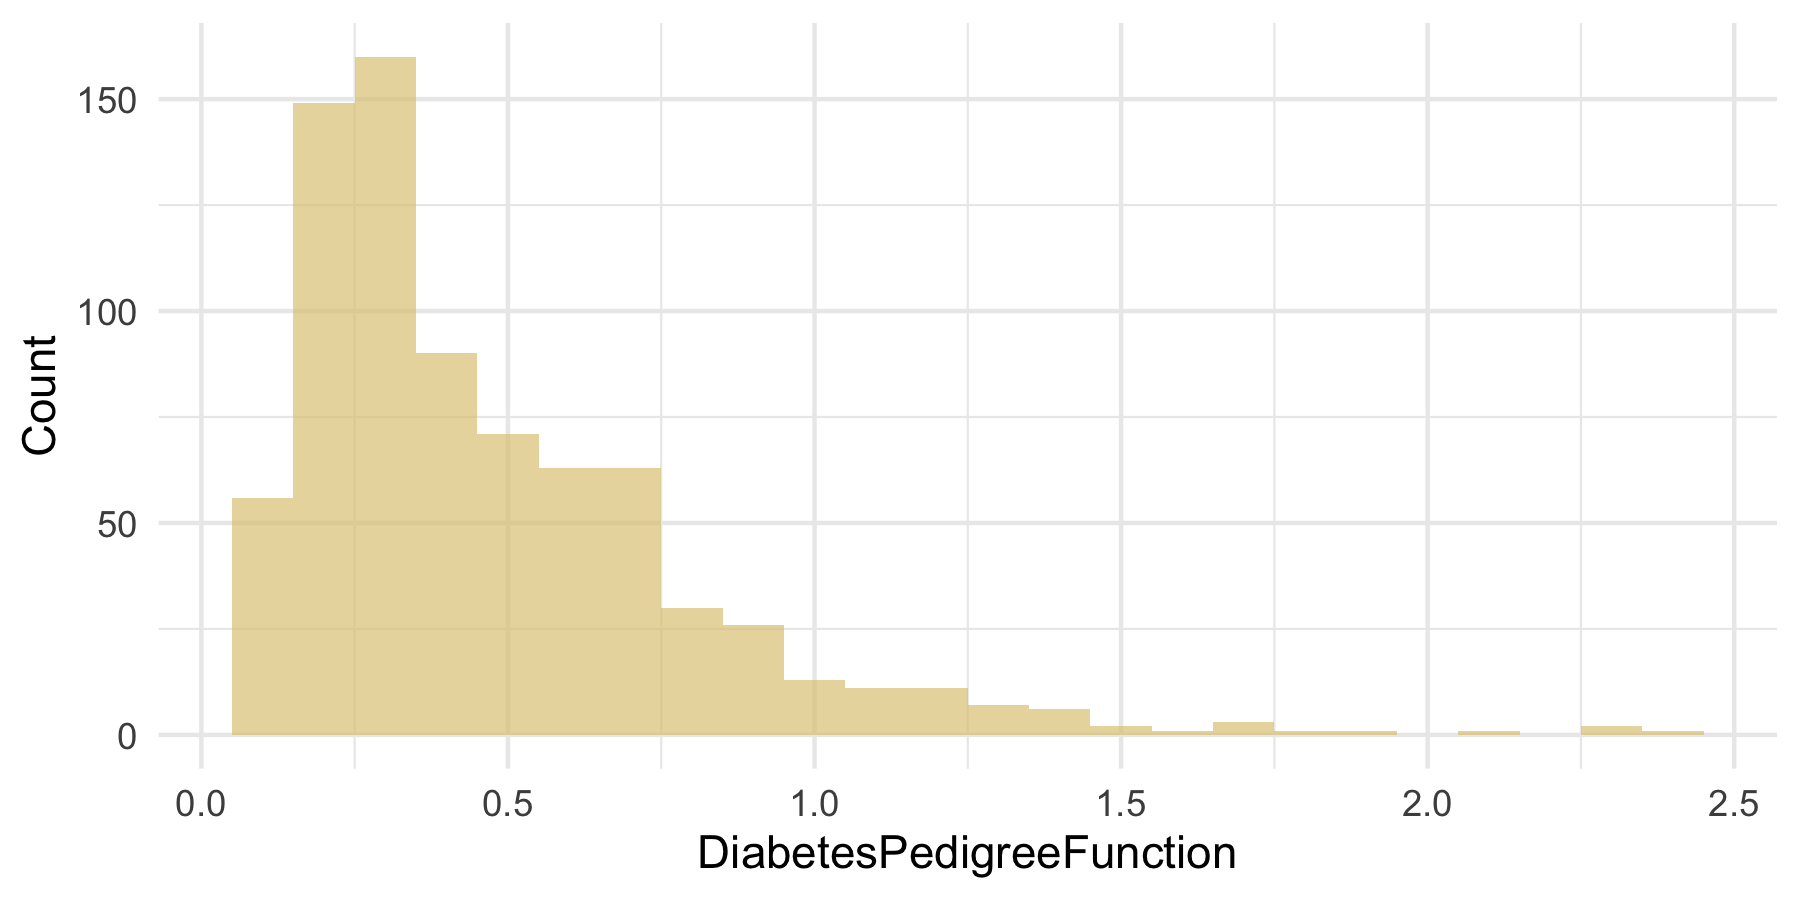
\includegraphics[width=0.65\textwidth]{img/pima-diab-ped-function.png}
    \end{center}
    \newpage
  \item Age
    \begin{center}
    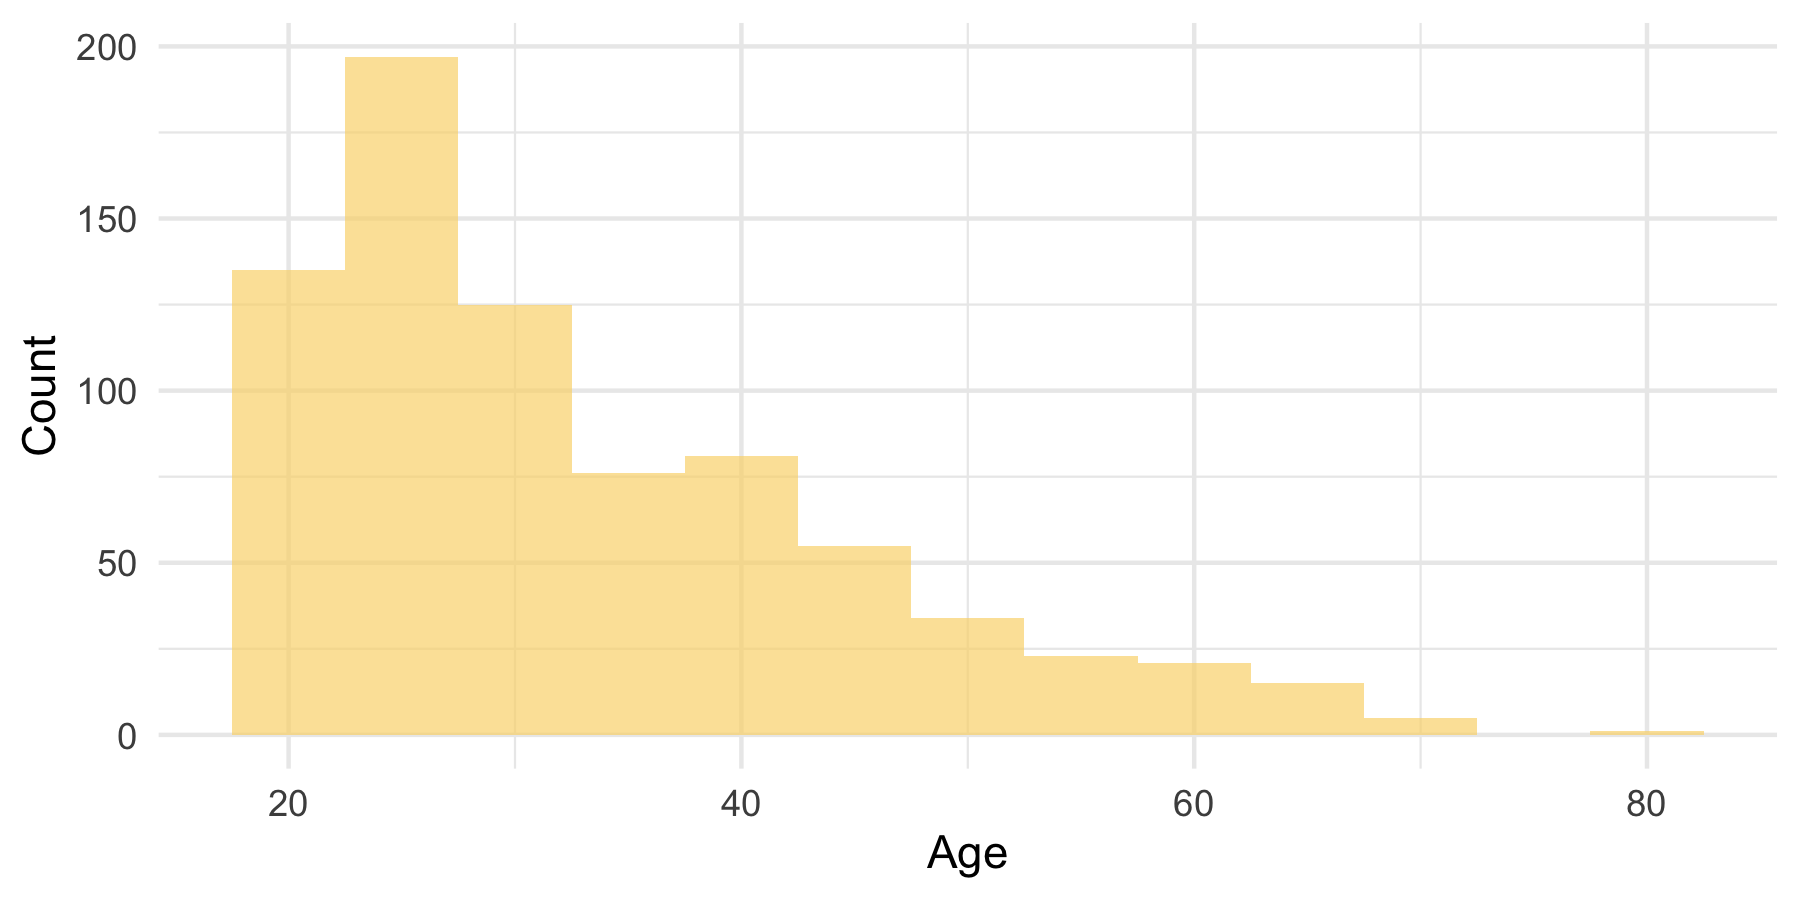
\includegraphics[width=0.65\textwidth]{img/pima-age.png}
    \end{center}
  \end{enumerate}
\end{question}

\begin{question}{}
The type of study design here is called a \textbf{prospective cohort study}. How would you collect information on these eight predictors if this were a \textbf{retrospective cohort study} (e.g., if you collected information about these women and their subsequent development of diabetes from the EHR)? How might this change affect how you extract and code the predictors? 
\end{question}

\subsection{Transformations}

Depending on the learning algorithm you're using and the goal of your project, you may or may not decide to employ transformations. A \textbf{transformation} is simply the application of a deterministic mathematical function to your data. In a supervised learning problem, you can transform one or more of the predictors and/or the outcome. Transformations are used to improve the interpretability of the model and/or to ensure that the model fulfills the assumptions of the statistical inference method(s) being used (e.g., a hypothesis test).

For example, here is what happens to the ``diabetes pedigree function'' predictor in the Pima dataset when we employ a common transformation called a \textbf{log transformation}\footnote{Here we are using log base 10, but you could also perform a similar transformation with the natural log, $\log_2$, etc.}:

\begin{center}
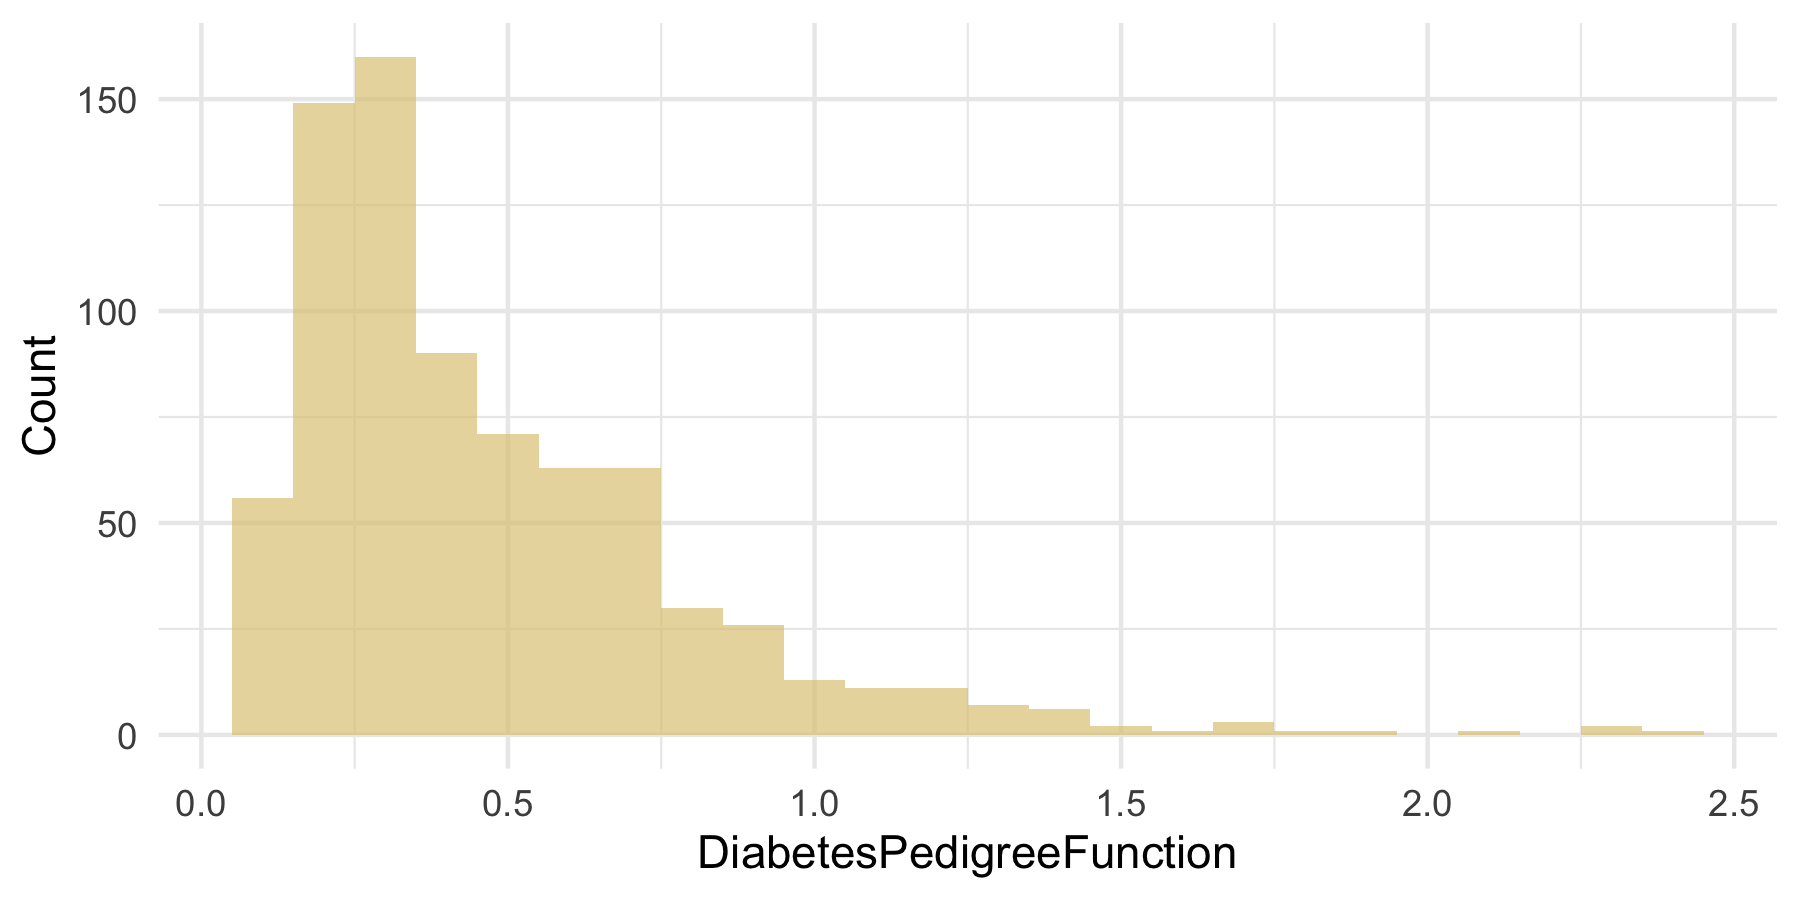
\includegraphics[width=0.49\textwidth]{img/pima-diab-ped-function.png} 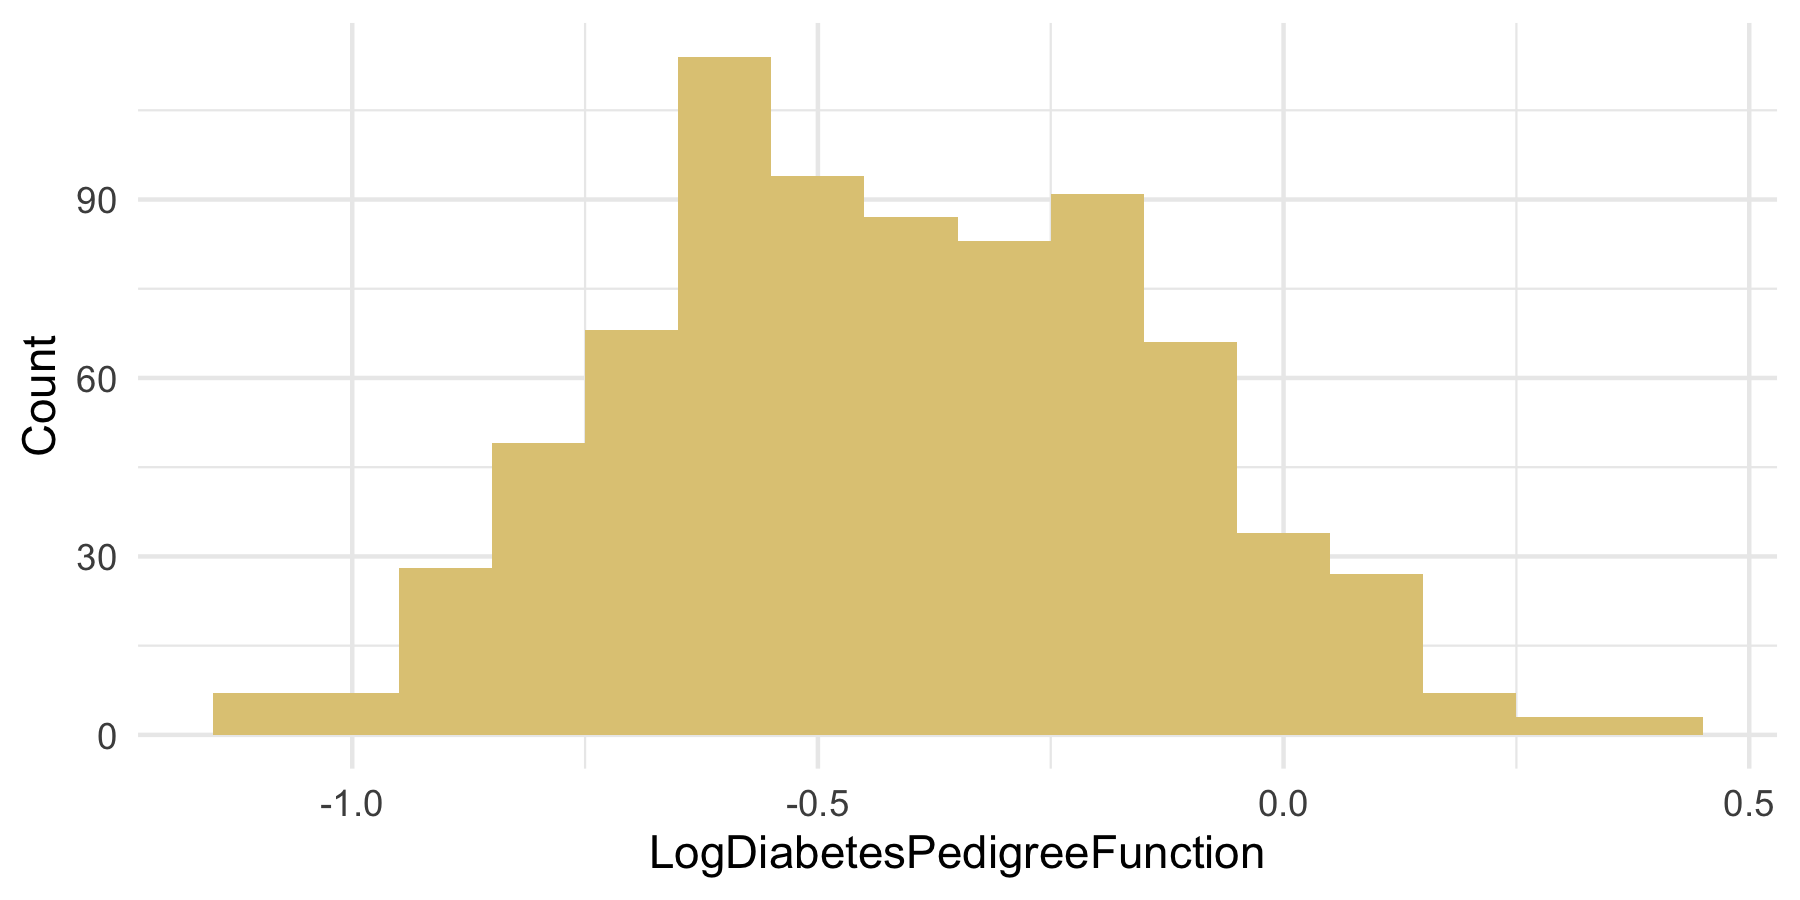
\includegraphics[width=0.49\textwidth]{img/pima-diab-ped-function-log.png}
\end{center}

\begin{question}{}
In the log transformation shown here, we simply replace each value, $x$, by $\log_{10}(x)$. Every unit increase on a $\log_{10}$ scale corresponds to a 10-fold multiplication on the usual scale of the predictor. If you put the log-transformed predictor into a regression model in place of the original (linear is the easiest to understand, but you could also consider logistic, Poisson, etc.), how would that change your interpretation of the model? 
\end{question}

Political science, economics, sociology, and related disciplines, which are heavily dependent on the use of linear regression models and hypothesis tests, rely extensively on transformations. In my experience, machine learning folks spend almost no time on them because their primary concern is predictive accuracy, not model interpretation. Machine learning practitioners, however, very frequently \textbf{scale and center} their predictors (see footnote in Section~\ref{section:sehyp}), which is another type of transformation. We will get into more detail on transformations as we continue to learn about regression models. 

\subsection{Correlations and Redundancy \label{section:redund}}

Including dozens or hundreds of predictors in a model does not guarantee that each contributes independent information. A good rule of thumb for any model is that it should be \textbf{parsimonious}: it should accomplish its goal with as little complexity and as few parameters as possible.

Finding a parsimonious model often means identifying sources of redundancy in a dataset. Often, two or more variables will be \textbf{correlated}, meaning that the value of one provides at least some information about the value of the other(s). A good way to alert yourself to the presence of highly correlated predictors is to create some sort of \textbf{correlogram}, or scatterplot matrix, which looks at associations between all pairs of variables. A correlogram for the Pima dataset is below.

\begin{center}
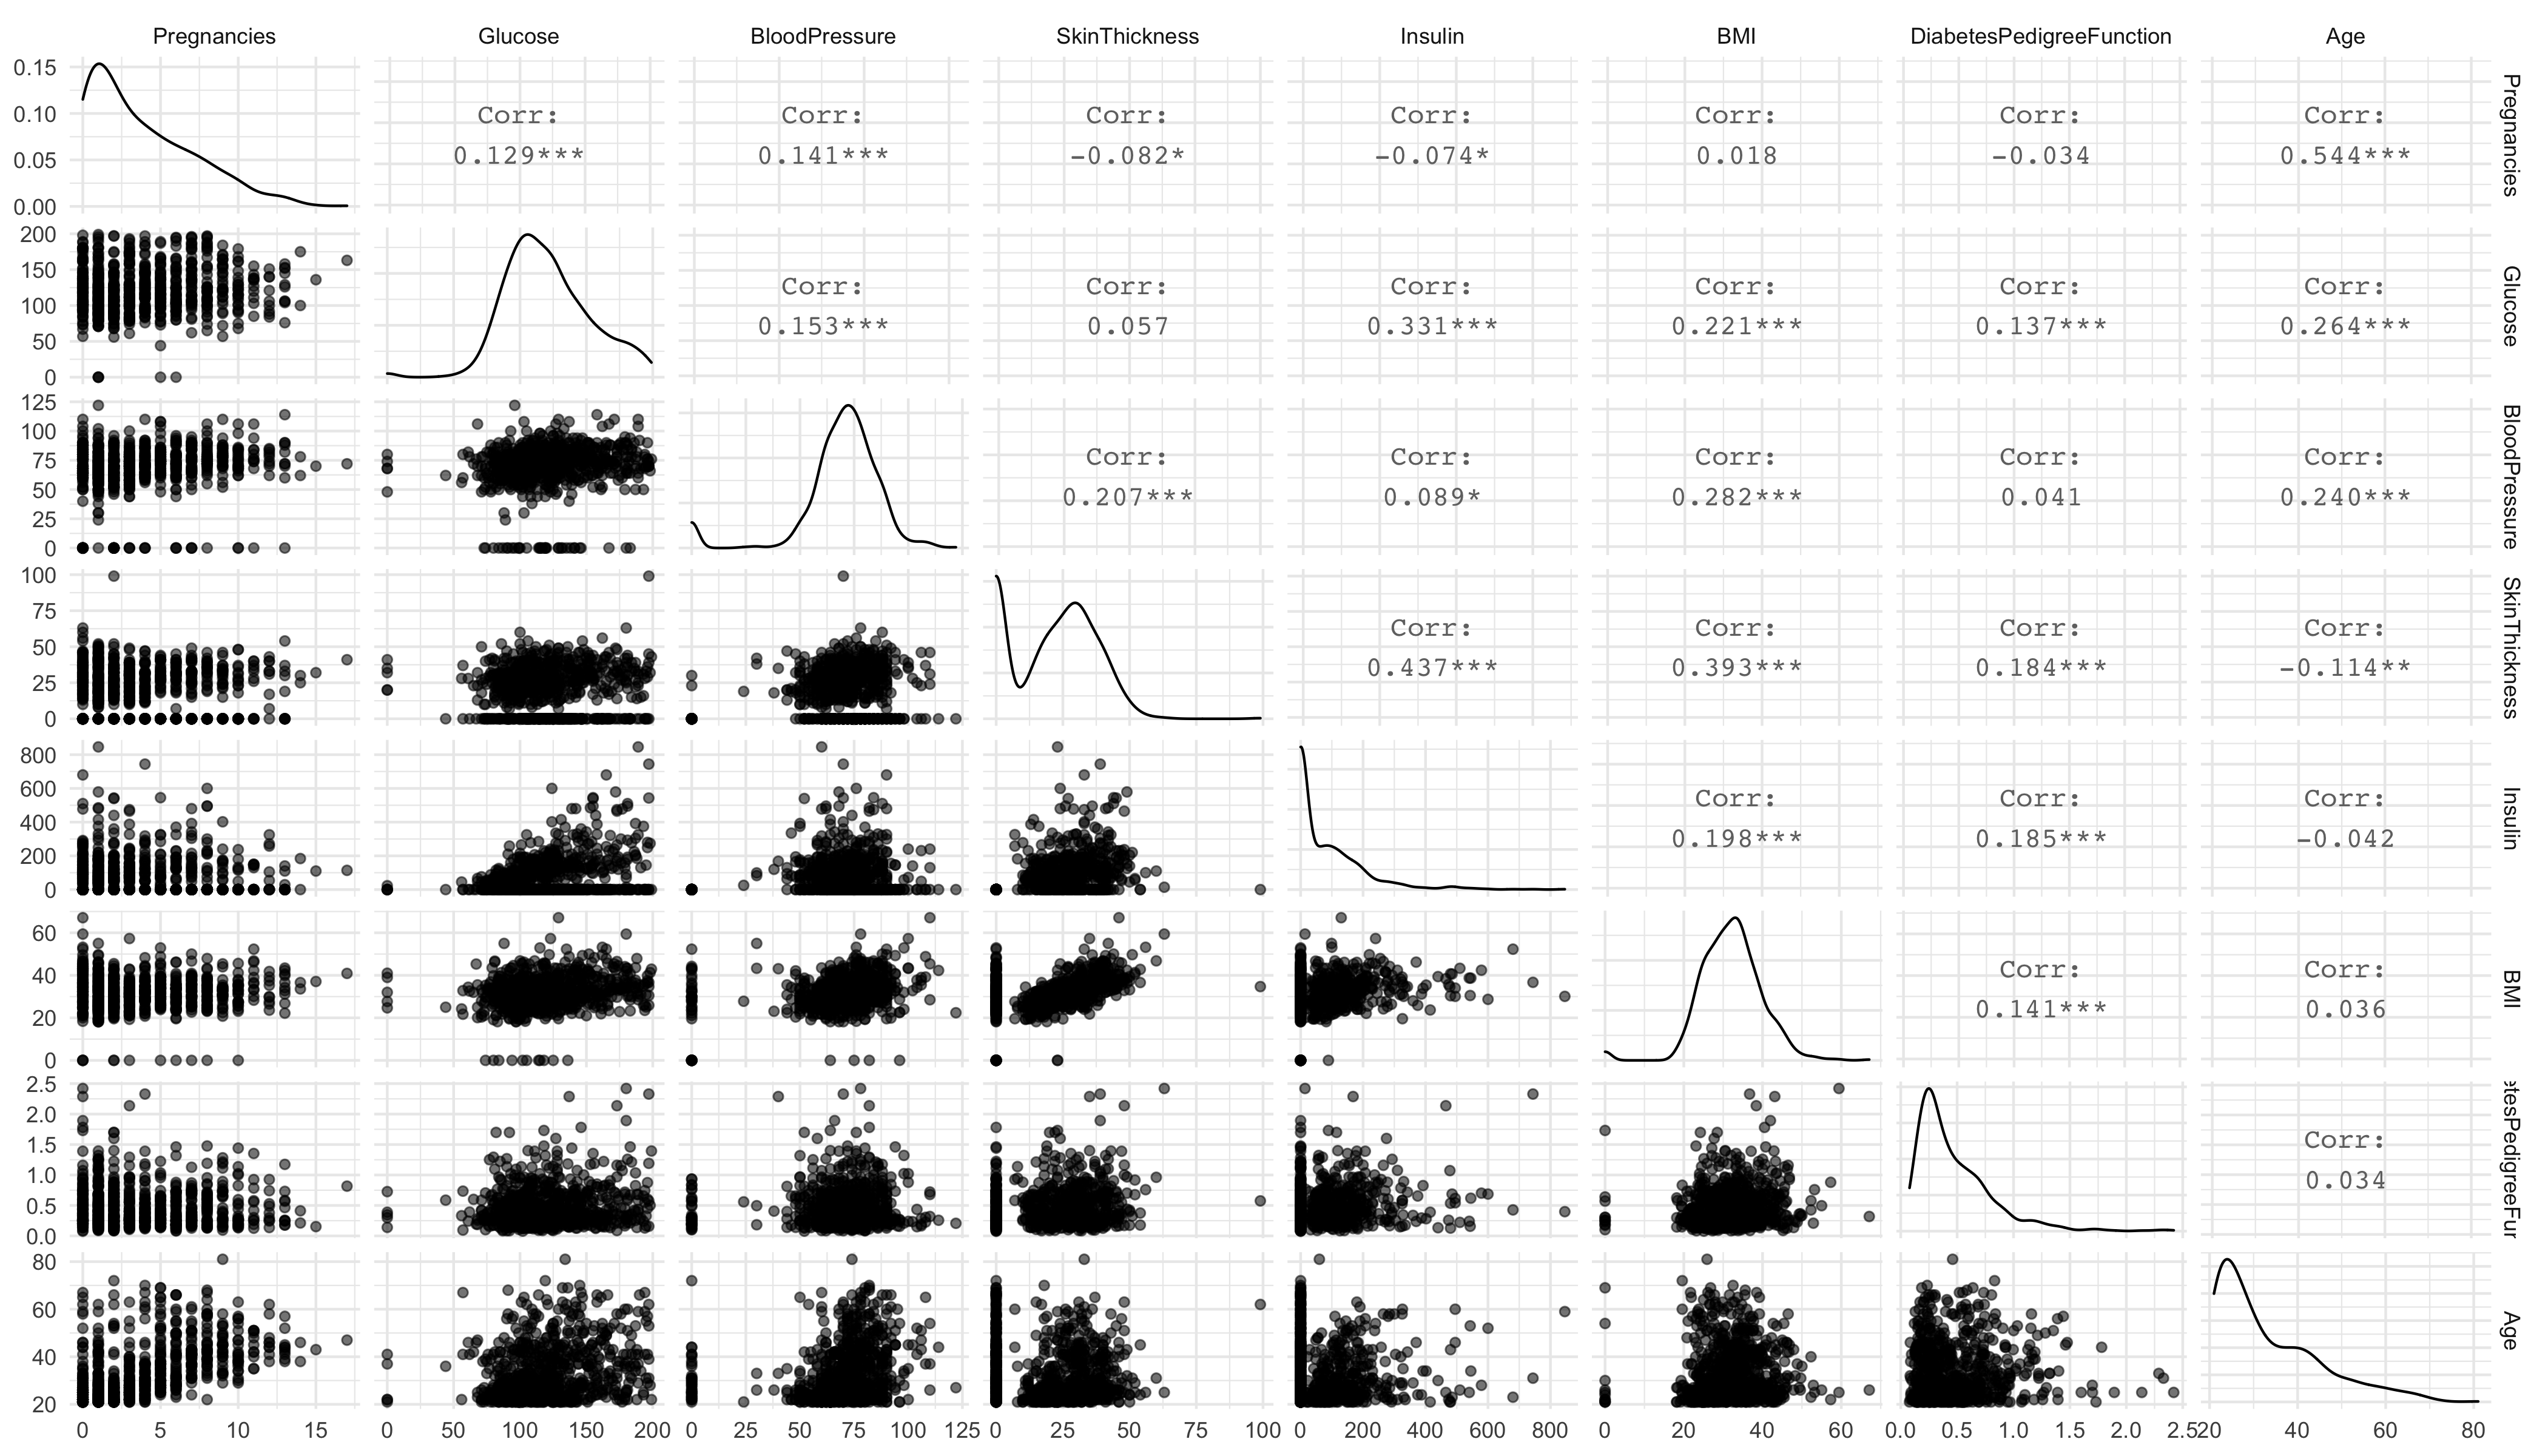
\includegraphics[width=\textwidth]{img/pima-ggpairs.png}
\end{center}

\begin{question}{}
This correlogram quantifies correlation using a metric called the \textbf{Pearson correlation coefficient}. Which pairs of predictors are the most tightly correlated? Are they positively or negatively correlated? How might you modify your dataset to eliminate redundancies in the information contributed by the different predictors?
\end{question}

Including correlated predictors is not always a bad thing, especially if your goal is prediction rather than model interpretation (see \cite{guyon2003introduction}, Figures 1, 2, and 3). The presence of correlations will also affect different types of models in different ways, and some suffer more than others. 

For example, here are eight univariate logistic regression models that capture the effect of each predictor in the Pima dataset on the outcome of diabetes vs. no diabetes:

\begin{center}
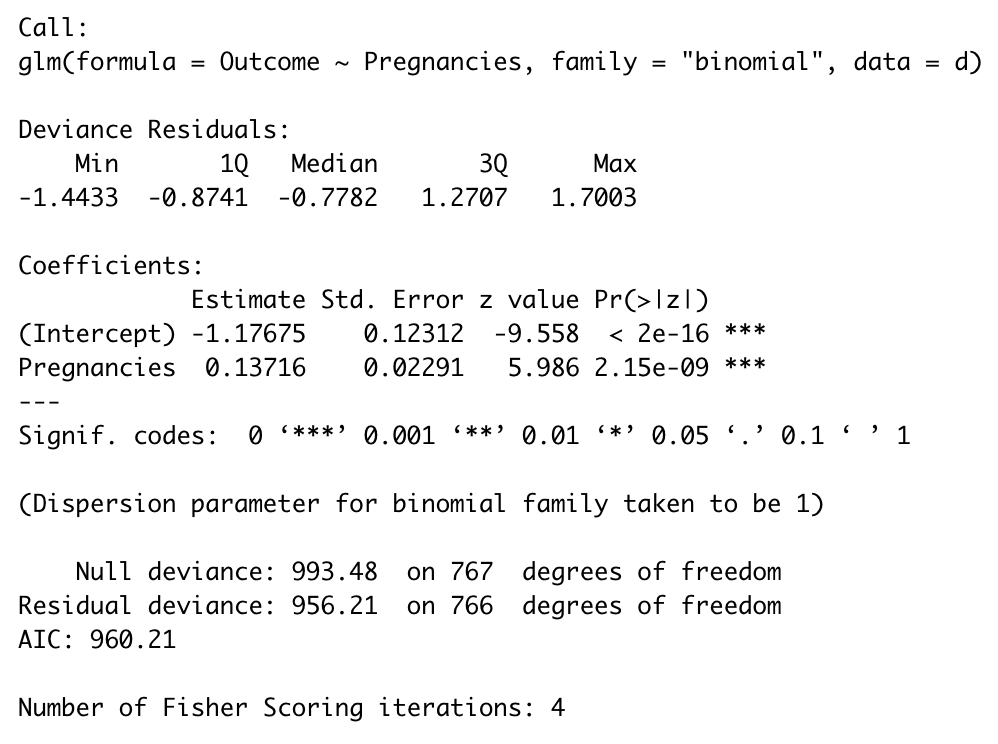
\includegraphics[width=0.45\textwidth]{img/cor-example-pregnancies.png}
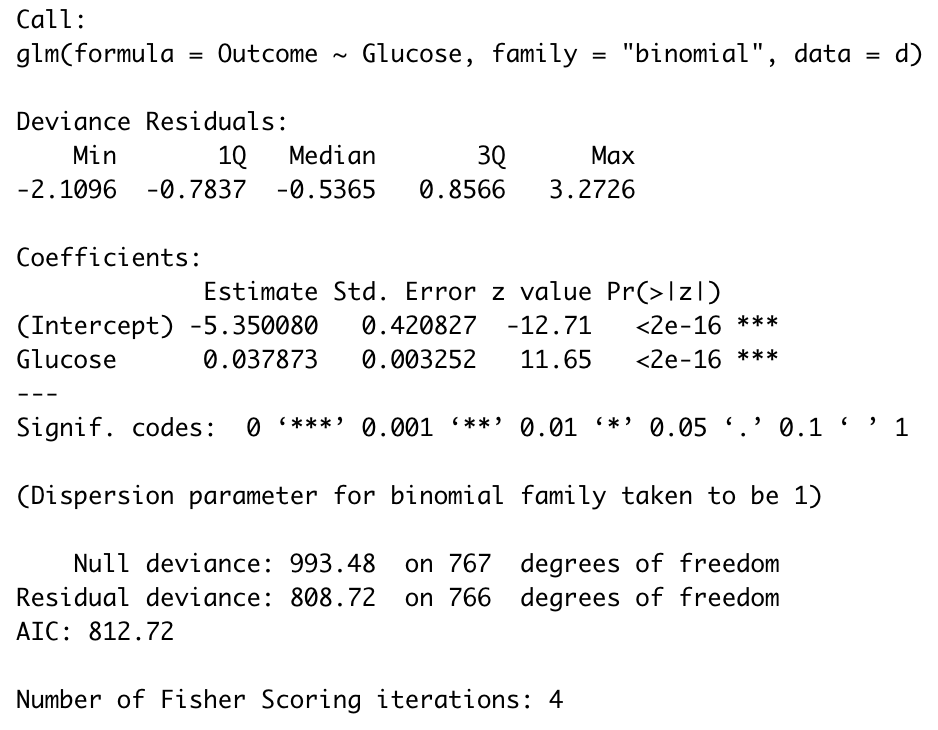
\includegraphics[width=0.45\textwidth]{img/cor-example-glucose.png} \\[2mm]
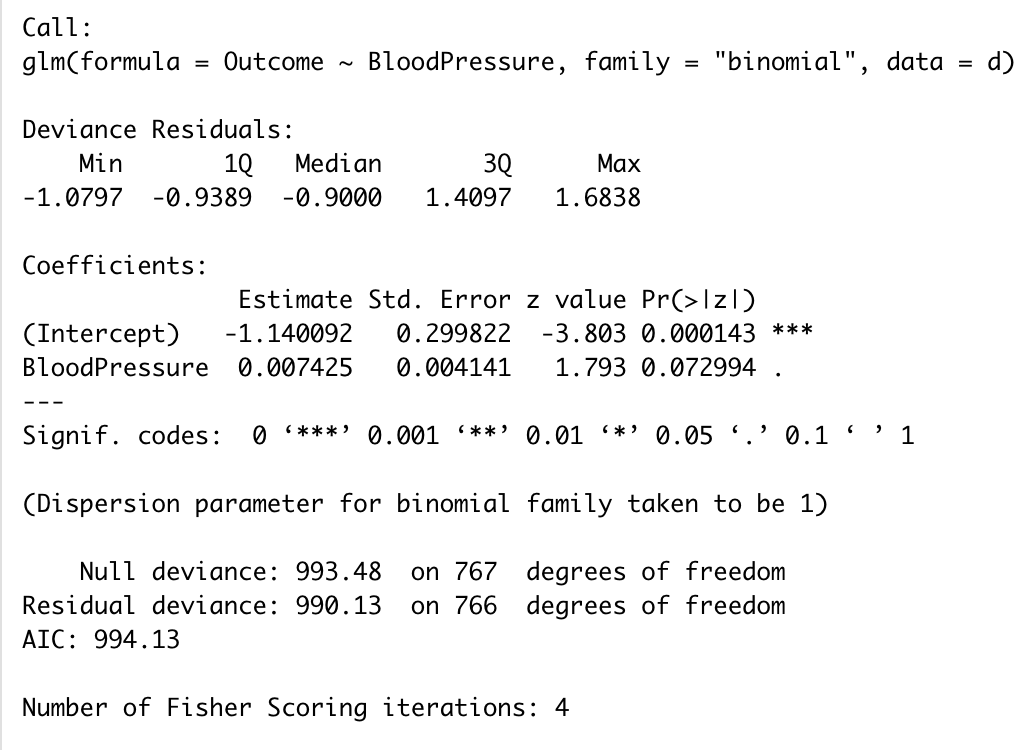
\includegraphics[width=0.45\textwidth]{img/cor-example-bp.png}
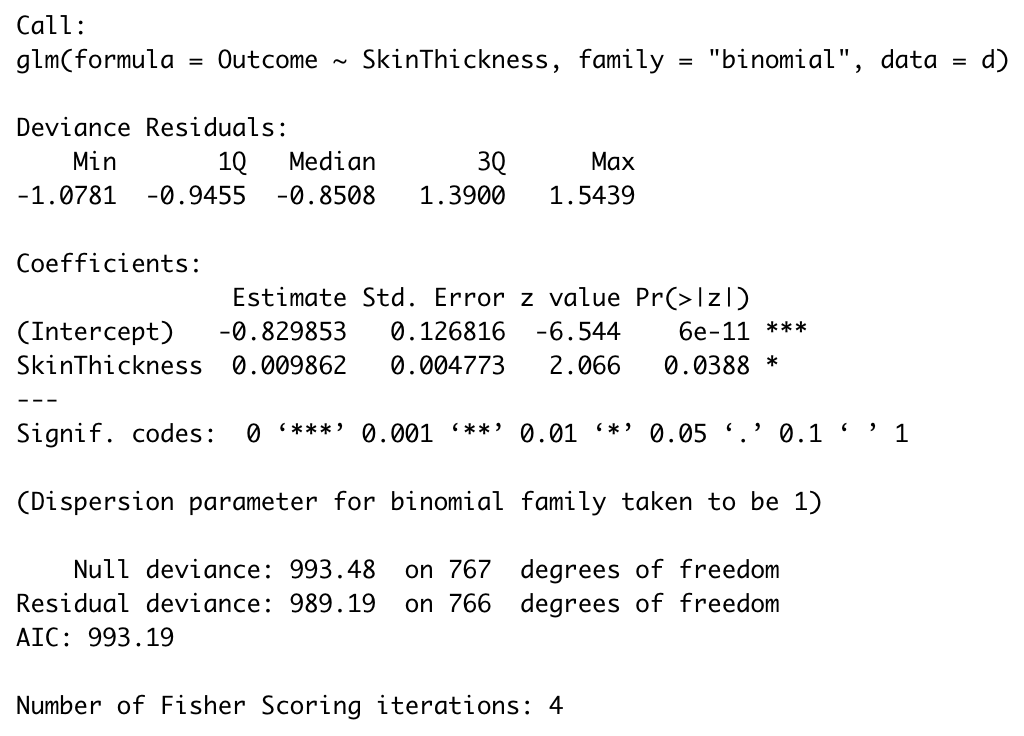
\includegraphics[width=0.45\textwidth]{img/cor-example-skin-thickness.png} \\[2mm]
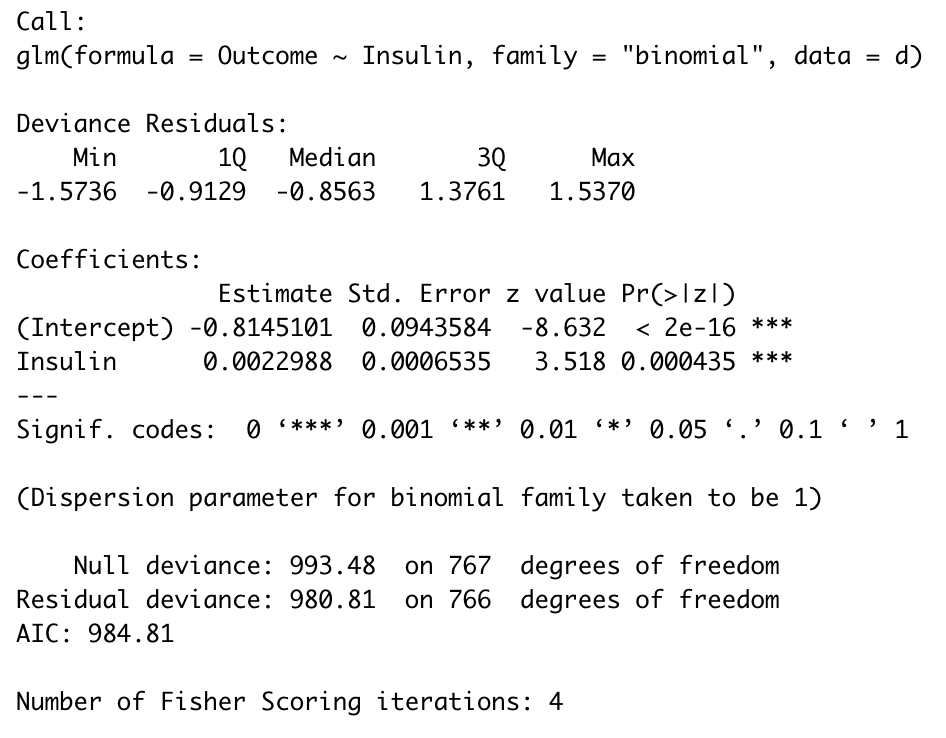
\includegraphics[width=0.45\textwidth]{img/cor-example-insulin.png}
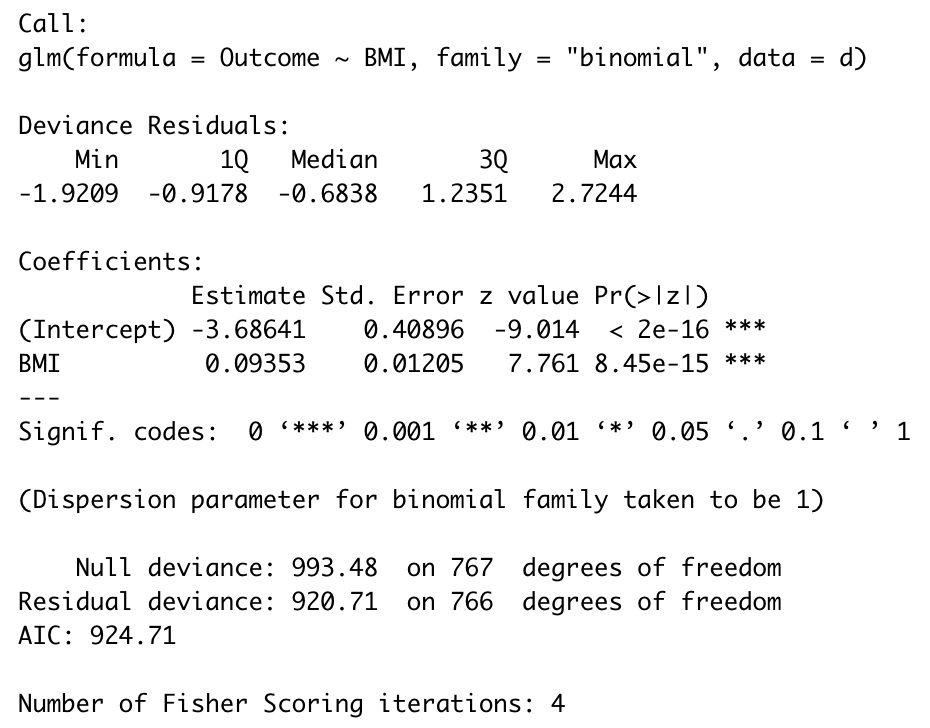
\includegraphics[width=0.45\textwidth]{img/cor-example-bmi.png} \\[2mm]
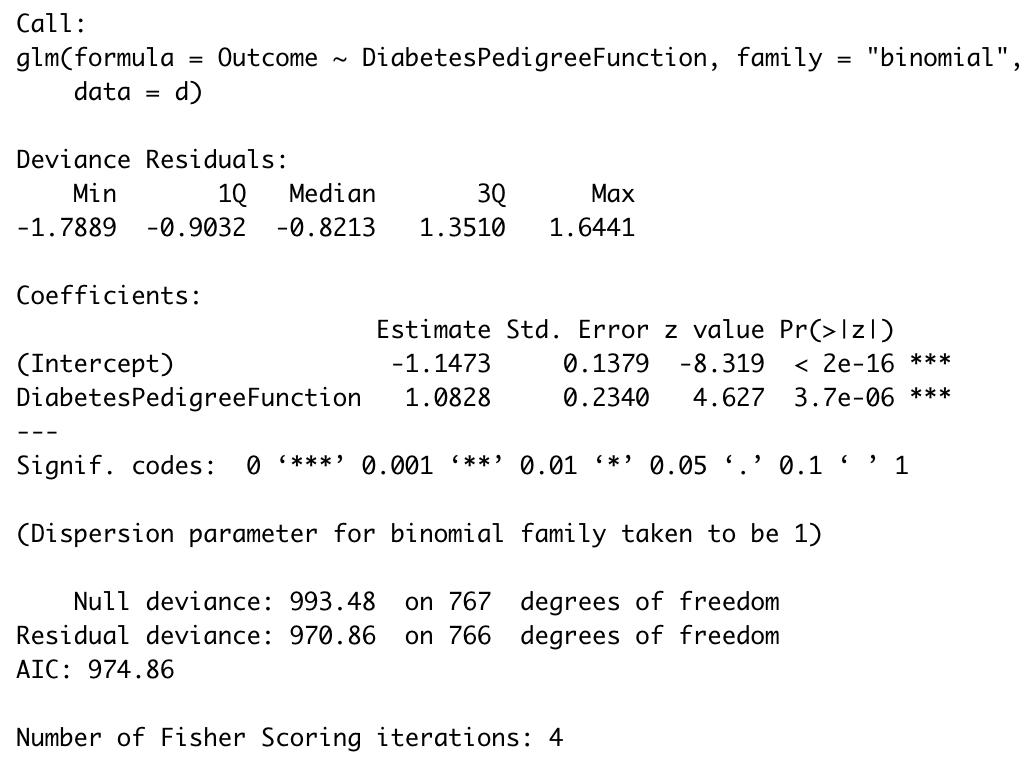
\includegraphics[width=0.45\textwidth]{img/cor-example-diab-ped-funct.png}
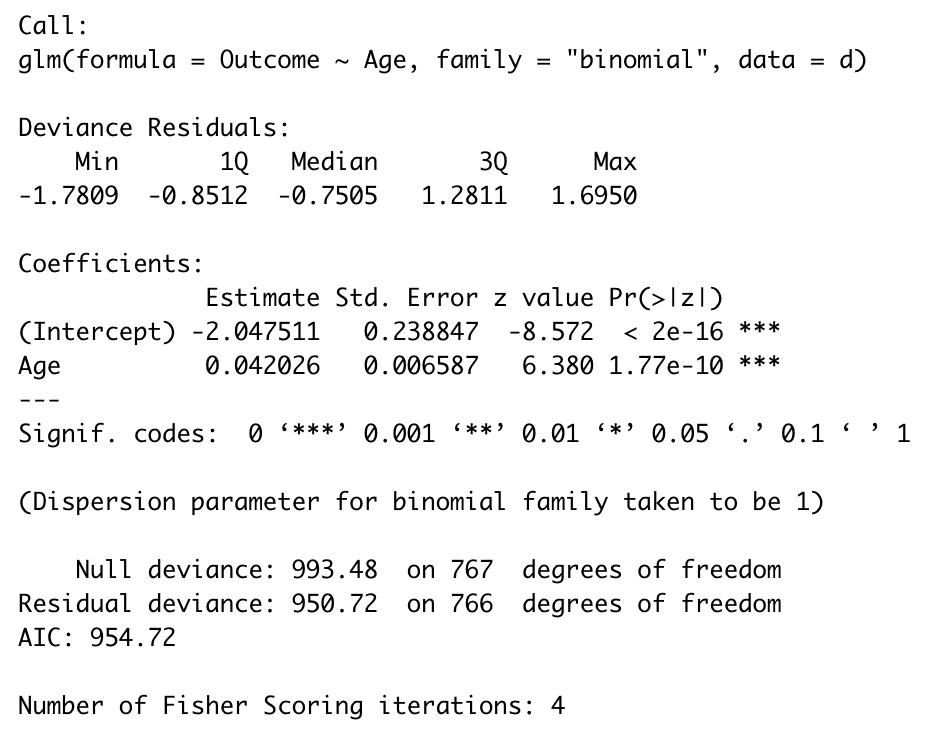
\includegraphics[width=0.45\textwidth]{img/cor-example-age.png}
\end{center}

The coefficients on each predictor here are called the \textbf{unadjusted coefficients}, and the p-values on the predictor-specific hypothesis tests are called  \textbf{unadjusted p-values}. If you exponentiate a coefficient in a univariate logistic regression model, you get an \textbf{unadjusted odds ratio}\footnote{See Chapter~\ref{chapter:glms} if you don't understand why you're exponentiating or where the term ``odds ratio'' comes from. The odds ratio compares the odds of having a positive outcome among two groups separated by a one unit difference of the predictor in question, all else being the same.}. Here is a summary table:
\vspace{-3mm}

\begin{center} 
\texttt{ \small
\begin{tabular}{llll}
\toprule
Predictor & Unadjusted  & Unadjusted  & Unadjusted  \\
& Coefficient & Odds Ratio & P-value \\
\midrule
Pregnancies & 0.137 & 1.147 & $<$0.001 \\
Glucose & 0.038 & 1.039 & $<$0.001 \\
BloodPressure & 0.007 & 1.007 & 0.073 \\
SkinThickness & 0.010 & 1.010 & 0.039 \\
Insulin & 0.002 & 1.002 & $<$0.001 \\
BMI & 0.094 & 1.100 & $<$0.001 \\
DiabetesPedigreeFunction & 1.083 & 2.953 & $<$0.001 \\
Age & 0.042 & 1.043 & $<$0.001 \\
\bottomrule
\end{tabular}
}
\end{center}

Now let's create one big logistic regression model that includes all eight predictors. This is called a \textbf{multivariate} model. The coefficients, exponentiated coefficients, and p-values are often called \textbf{adjusted} in this case, or one might say that the odds ratio measures the effect of one predictor, \textbf{controlling for} the effects of the other predictors. Here are the adjusted estimates:
\vspace{-3mm}
\begin{center} 
\texttt{ \small
\begin{tabular}{llll}
\toprule
Predictor & Adjusted  & Adjusted  & Adjusted  \\
& Coefficient & Odds Ratio & P-value \\
\midrule
Pregnancies & 0.123 & 1.131 & $<$0.001 \\
Glucose & 0.035 & 1.036 & $<$0.001 \\
BloodPressure & -0.013 & 0.987 & 0.011 \\
SkinThickness & 0.001 & 1.001 & 0.929 \\
Insulin & -0.001 & 0.999 & 0.186 \\
BMI & 0.090 & 1.094 & $<$0.001 \\
DiabetesPedigreeFunction & 0.945 & 2.573 & 0.002 \\
Age & 0.015 & 1.015 & 0.111 \\
\bottomrule
\end{tabular}
}
\end{center}

\begin{question}{}
How can the odds ratio for Insulin be so close to 1.0 yet its p-value so low? (Hint: See Section~\ref{section:sehyp}.)
\end{question}

\begin{question}{}
Why might the coefficient and p-value for SkinThickness change so much in the shift from unadjusted to adjusted? 
\end{question}


%%%%%%%%%%%%%%%%%%%%%%%%%%%%%%%%%%%%%%%%%%%%%%%%%%%%%%%%%%%%%%%%%%%%%%

\section{Feature Selection}

The process of feature selection is largely about eliminating redundancies and useless predictors in an effort to come up with the most parsimonious model possible. In many cases, it is also about increasing the accuracy of model interpretation. There are three basic approaches to feature selection: filters, wrappers, and embedded methods. 

\subsection{Filters}

\textbf{Filter methods} select subsets of variables as a preprocessing step, \emph{independently of the chosen model}. These methods use \textbf{proxy measures} to rank variables; the proxy measure is often chosen to be computationally fast so that large numbers of features can be sifted through quickly.

A predetermined threshold of the proxy measure is usually used to determine which features pass to the multivariate modeling stage. Alternatively, the modeler may decide on a fixed number of features to include. Some examples of filter methods include:

\begin{itemize}
\item Any kind of univariate model (e.g. univariate logistic or linear regression)
\item Any kind of hypothesis test (e.g. t-test, chi-squared test; see Chapter~\ref{chapter:hypothesistesting})
\item Any kind of correlation coefficient (e.g. Pearson, Spearman)
\item Mutual information\footnote{The mutual information, in another format, is the most common splitting criterion used for decision trees; see Chapter~\ref{chapter:decisiontrees}. In the case of continuous variables, the sums are replaced by integrals.} 
$$ MI(X_i,Y) = \sum_x \sum_y P(X_i = x, Y = y) \log \frac{P(X_i = x, Y = y)}{P(X_i = x) P(Y = y)} $$
\item Variance thresholding (simply remove features with low variance)
\end{itemize}

\begin{question}{}
If you wanted to use the univariate logistic regression models above in Section~\ref{section:redund} as a filter for a downstream model (potentially not even multivariate logistic regression - it could be a decision tree, etc.), how would you rank them and how would you decide on an appropriate cutoff? 
\end{question}

\begin{question}{}
How would you apply a filter-based selection method in a case where you had dozens of different predictors of different types (e.g. some categorical, some binary, some numeric)? 
\end{question}

\begin{question}{}
How might you choose the appropriate threshold for a filter-based method in a data-driven way? 
\end{question}

\begin{question}{}
What is problematic about testing each potential feature, one at a time?
\end{question}

\subsection{Wrappers}

\textbf{Wrapper methods} use a search algorithm to traverse the space of possible features, evaluating each subset by running the chosen model using that subset. They are generally computationally intensive (e.g., imagine trying to find the optimal subset of 10,000 features, or even 50) so \textbf{heuristics} generally have to be used to pare down the search space. Some examples of wrapper methods include:

\begin{itemize}
\item \textbf{Exhaustive search.} Try all possible subsets of features. If there are $m$ features, this means trying $2^m$ possible subsets.
\item \textbf{Forward selection.} Start with a baseline (e.g., intercept only) model. Add in each of $m$ possible predictors individually and take the best one based on some performance criterion. Repeat, adding one predictor at each step, until the performance criterion stops getting better or you run out of predictors. 
\item \textbf{Backward elimination.} Start with a complete model (all predictors included). Try removing each predictor and take the one whose removal causes the performance criterion to increase the most. Repeat, removing one predictor at each step, until the performance criterion stops getting better or you are left with no predictors (null model). 
\item \textbf{Forward-backward selection.} A combination of forward selection and backward elimination. 
\item \textbf{Simulated annealing.} Add or remove predictors with some probability depending on how well the model is doing. At each stage, if the new model is better, accept it; it becomes the new baseline. If the new model is worse, accept it with some probability, $p$, that decreases over time according to a ``cooling schedule''. This helps prevent the variable selection process from getting stuck in local optima. 
\end{itemize}

\begin{question}{}
Why is exhaustive search problematic for almost any reasonably sized $m$?
\end{question}

\vspace{2mm}

\begin{question}{}
Here is the output of forward selection for the Pima example, using R's \emph{MASS} package and the \textbf{Akaike Information Criterion (AIC)} as the model performance metric.
{\footnotesize
\begin{verbatim}
Start:  AIC=995.48
Outcome ~ 1
                           Df Deviance    AIC
+ Glucose                   1   808.72 812.72
+ BMI                       1   920.71 924.71
+ Age                       1   950.72 954.72
+ Pregnancies               1   956.21 960.21
+ DiabetesPedigreeFunction  1   970.86 974.86
+ Insulin                   1   980.81 984.81
+ SkinThickness             1   989.19 993.19
+ BloodPressure             1   990.13 994.13
<none>                          993.48 995.48

Step:  AIC=812.72
Outcome ~ Glucose

                           Df Deviance    AIC
+ BMI                       1   771.40 777.40
+ Pregnancies               1   784.95 790.95
+ DiabetesPedigreeFunction  1   796.99 802.99
+ Age                       1   797.36 803.36
<none>                          808.72 812.72
+ SkinThickness             1   807.07 813.07
+ Insulin                   1   807.77 813.77
+ BloodPressure             1   808.59 814.59

Step:  AIC=777.4
Outcome ~ Glucose + BMI

                           Df Deviance    AIC
+ Pregnancies               1   744.12 752.12
+ Age                       1   755.68 763.68
+ DiabetesPedigreeFunction  1   762.87 770.87
+ Insulin                   1   767.79 775.79
+ BloodPressure             1   769.07 777.07
<none>                          771.40 777.40
+ SkinThickness             1   770.20 778.20

Step:  AIC=752.12
Outcome ~ Glucose + BMI + Pregnancies

                           Df Deviance    AIC
+ DiabetesPedigreeFunction  1   734.31 744.31
+ BloodPressure             1   738.43 748.43
+ Age                       1   742.10 752.10
<none>                          744.12 752.12
+ Insulin                   1   742.43 752.43
+ SkinThickness             1   743.60 753.60

Step:  AIC=744.31
Outcome ~ Glucose + BMI + Pregnancies + 
          DiabetesPedigreeFunction

                Df Deviance    AIC
+ BloodPressure  1   728.56 740.56
+ Insulin        1   731.51 743.51
<none>               734.31 744.31
+ Age            1   732.51 744.51
+ SkinThickness  1   733.06 745.06

Step:  AIC=740.56
Outcome ~ Glucose + BMI + Pregnancies + 
          DiabetesPedigreeFunction + 
          BloodPressure

                Df Deviance    AIC
+ Age            1   725.46 739.46
+ Insulin        1   725.97 739.97
<none>               728.56 740.56
+ SkinThickness  1   728.00 742.00

Step:  AIC=739.46
Outcome ~ Glucose + BMI + Pregnancies + 
          DiabetesPedigreeFunction + 
          BloodPressure + Age

                Df Deviance    AIC
+ Insulin        1   723.45 739.45
<none>               725.46 739.46
+ SkinThickness  1   725.19 741.19

Step:  AIC=739.45
Outcome ~ Glucose + BMI + Pregnancies + 
          DiabetesPedigreeFunction + 
          BloodPressure + Age + Insulin

                Df Deviance    AIC
<none>               723.45 739.45
+ SkinThickness  1   723.45 741.45
\end{verbatim} 
}
What does the final model look like? Which predictor is missing from the final model? Note: AIC is an estimate of out-of-sample prediction error and depends on the likelihood; thus it does not work for models that do not calculate some form of likelihood.
\end{question}

\vspace{2mm}

\begin{question}{}
Here is the output of backward selection for the Pima example, again using R's \emph{MASS} package and AIC as the model performance metric.
{\footnotesize
\begin{verbatim}
Start:  AIC=741.45
Outcome ~ Pregnancies + Glucose + BloodPressure + SkinThickness + 
    Insulin + BMI + DiabetesPedigreeFunction + Age

                           Df Deviance    AIC
- SkinThickness             1   723.45 739.45
- Insulin                   1   725.19 741.19
<none>                          723.45 741.45
- Age                       1   725.97 741.97
- BloodPressure             1   729.99 745.99
- DiabetesPedigreeFunction  1   733.78 749.78
- Pregnancies               1   738.68 754.68
- BMI                       1   764.22 780.22
- Glucose                   1   838.37 854.37

Step:  AIC=739.45
Outcome ~ Pregnancies + Glucose + BloodPressure + Insulin + BMI + 
    DiabetesPedigreeFunction + Age

                           Df Deviance    AIC
<none>                          723.45 739.45
- Insulin                   1   725.46 739.46
- Age                       1   725.97 739.97
- BloodPressure             1   730.13 744.13
- DiabetesPedigreeFunction  1   733.92 747.92
- Pregnancies               1   738.69 752.69
- BMI                       1   768.77 782.77
- Glucose                   1   840.87 854.87
\end{verbatim}
}
What does the final model look like? How does it compare to the model obtained through forward selection?
\end{question}

\newpage

\subsection{Embedded Methods}

\textbf{Embedded methods} perform feature selection during the process of model training. They are usually specific to a particular type of model. 

One example of an embedded method is a decision tree (see Chapter~\ref{chapter:decisiontrees}), which implicitly performs feature selection by placing the most informative predictors at the top of the tree and ignoring those that are unassociated with the outcome. 

\vspace{2mm}

\begin{question}{}
Here is the decision tree produced by CART, using information gain/mutual information as the splitting criterion as usual:
\begin{center}
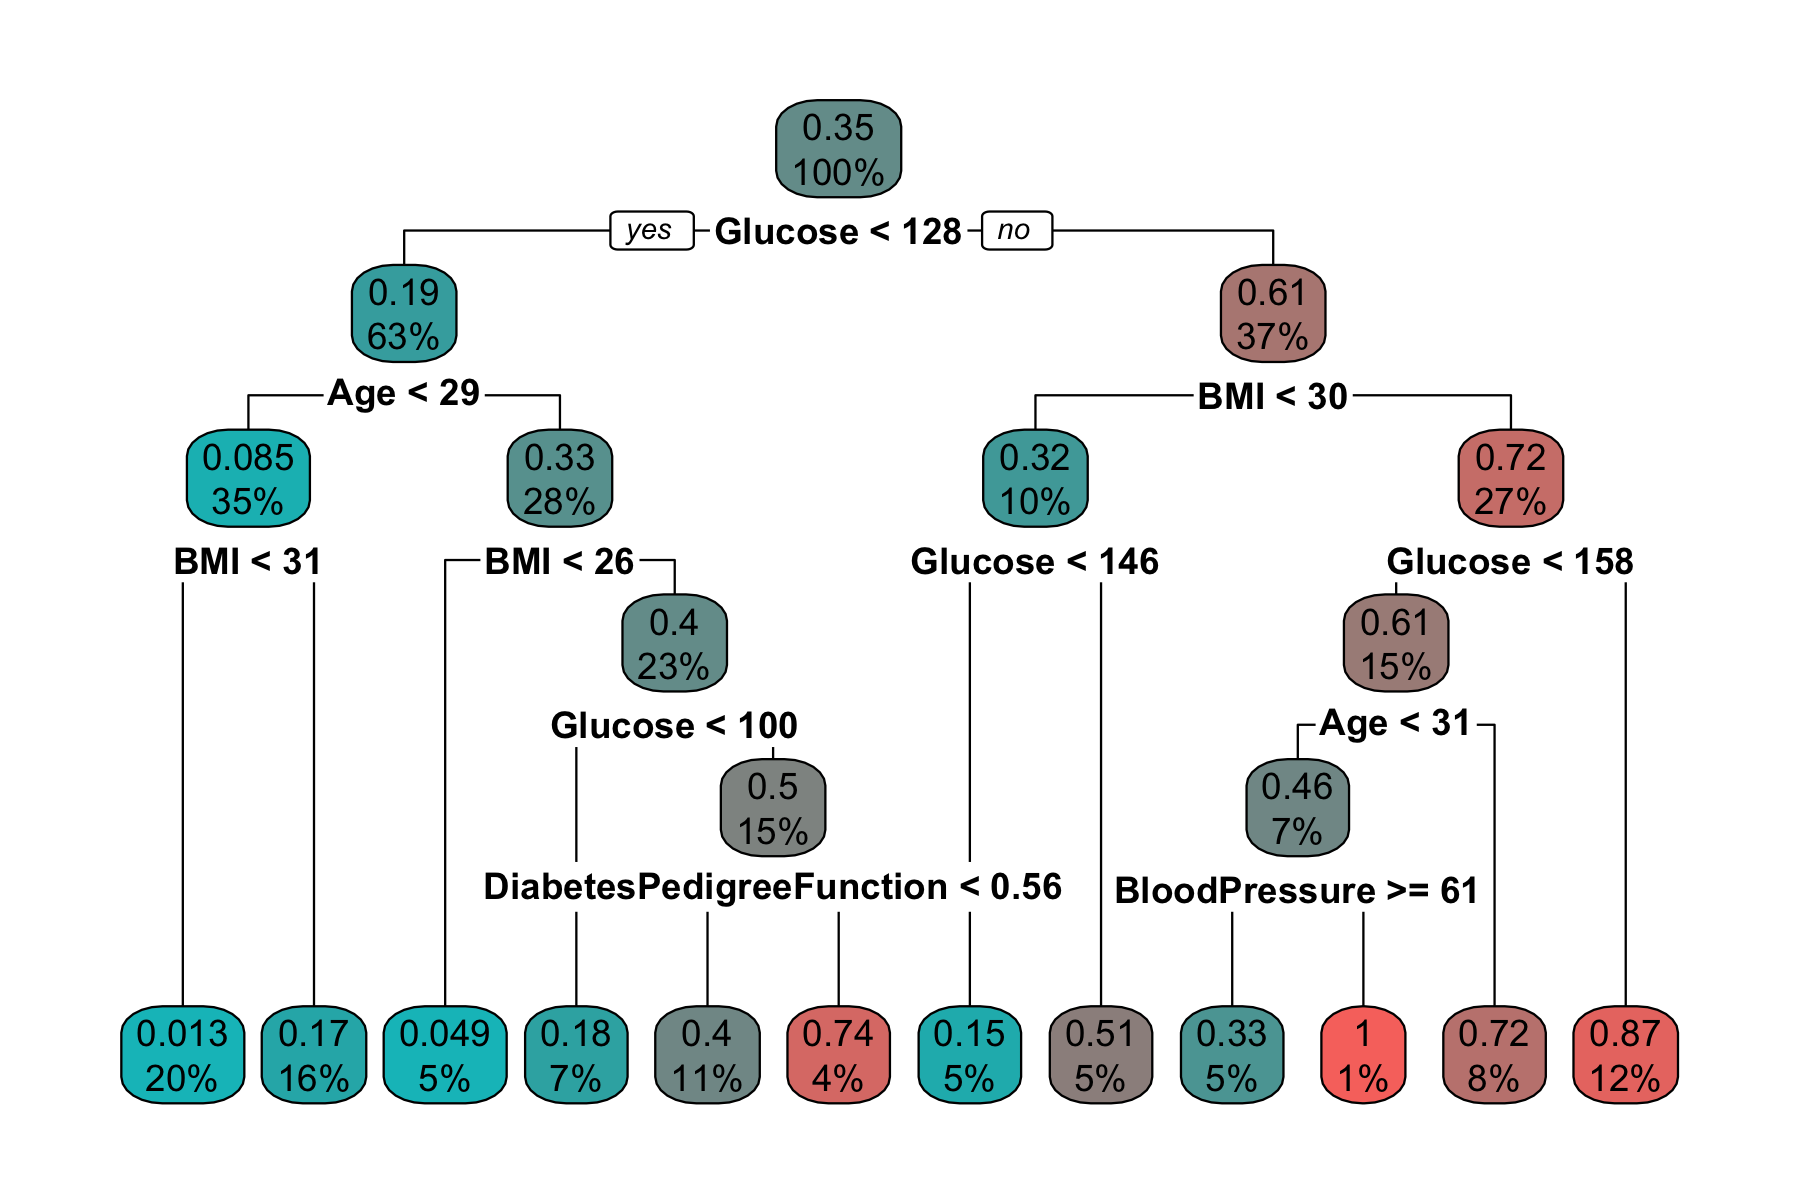
\includegraphics[width=\textwidth]{img/pima-decision-tree.png}
\end{center}
Which features were selected for this tree and which were ignored? How were the features transformed from their original forms in the dataset?
\end{question}

Another example of an embedded method is \textbf{regularization}. The easiest way to understand regularization is through our discussion of maximum likelihood estimation for GLMs in Chapter~\ref{chapter:glms}. The goal of maximum likelihood estimation is to find the set of model coefficients, $\beta$s, that maximize the joint probability (likelihood) of our observed data given the model. The trouble with this is that more complex models, with more parameters, will generally fit the data better: i.e. produce a higher likelihood.

Regularization addresses this by introducing a penalty term on the likelihood that is proportional to the size of the parameters. In $L_1$ regularization, a.k.a. \textbf{Lasso}, the penalty term is proportional to the absolute values of the coefficients. It looks like this:
$$ \lambda \sum_{j=1}^p \vert \beta_j \vert $$
where $p$ is the number of predictors. This creates a tradeoff in the model between the likelihood and the number of parameters. During optimization, the model will set the coefficients on predictors to zero if including those predictors does not sufficiently improve the likelihood. The relative importance of the penalty term and likelihood is adjusted using the parameter $\lambda$. We will see regularized regression methods in much greater detail in Chapter~\ref{chapter:lassoridge}. 

\begin{question}{}
Here is the raw model output from the multivariate logistic regression model that includes all eight predictors:
\begin{center}
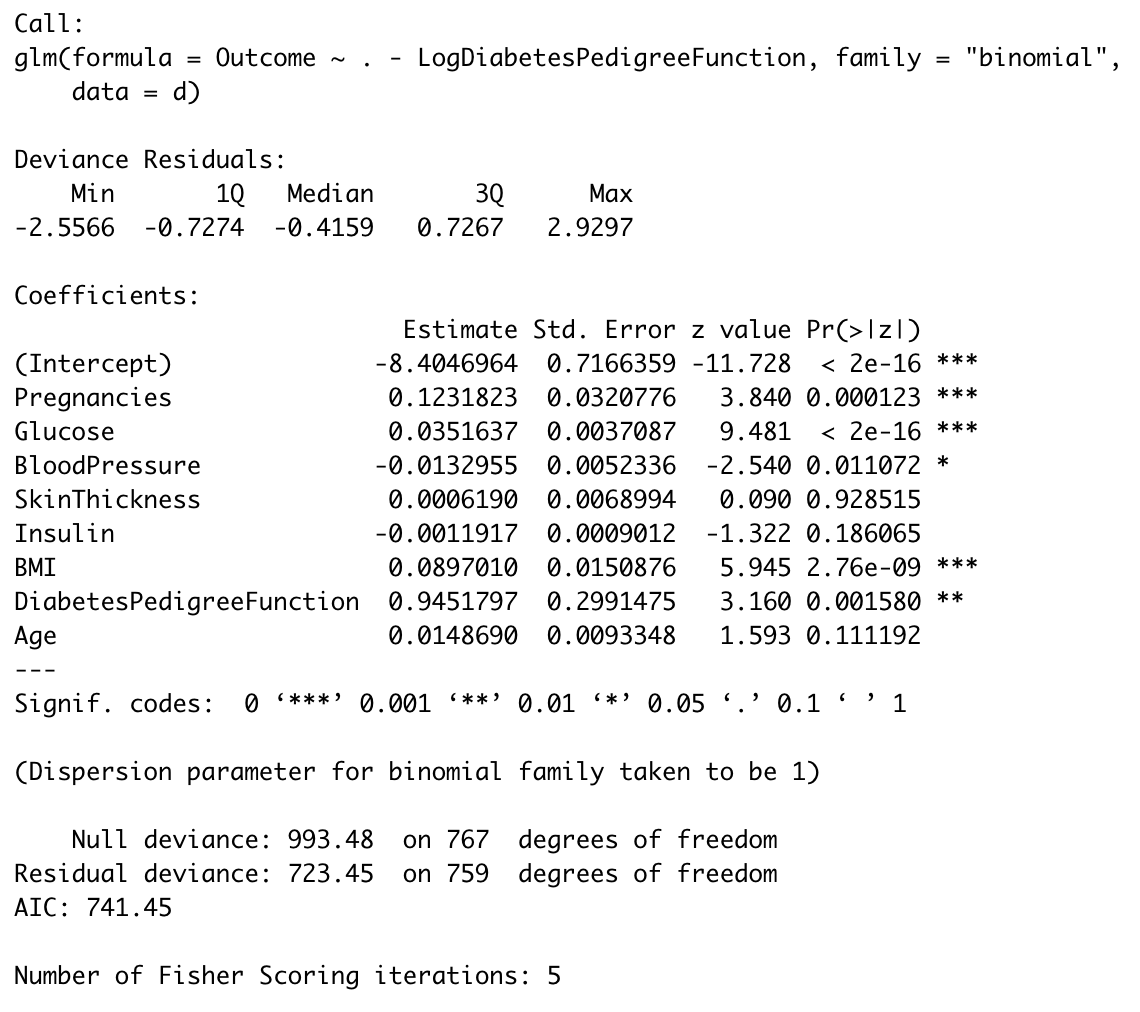
\includegraphics[width=0.7\textwidth]{img/cor-example-multivar.png}
\end{center}
Now let's consider what happens when we use a $L_1$ regularized logistic regression model, produced using the R package \emph{glmnet}. Here is what happens to the model's error (assessed using $10$-fold cross validation; measured using a metric called \textbf{binomial deviance}) when we vary $\lambda$:
\begin{center}
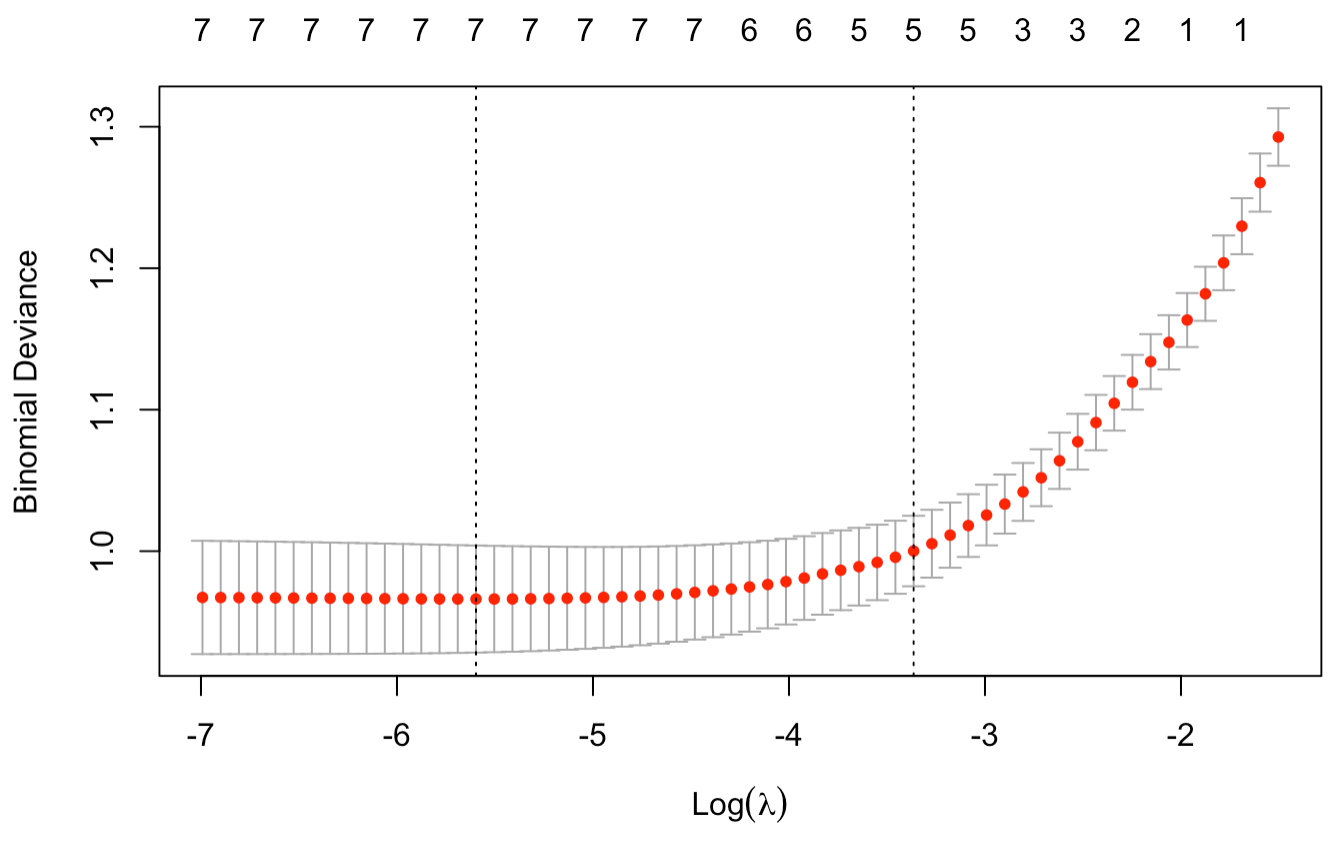
\includegraphics[width=0.8\textwidth]{img/pima-glmnet-plot.png}
{\small
\begin{verbatim}
Measure: Binomial Deviance 

      Lambda Measure      SE Nonzero
min 0.004468  0.9686 0.02647       7
1se 0.028723  0.9922 0.02118       5
\end{verbatim}
}
\end{center}
We choose $\lambda$ to be equal to the value that produces the minimum deviance. Here are the coefficients of the final model:
\begin{center}
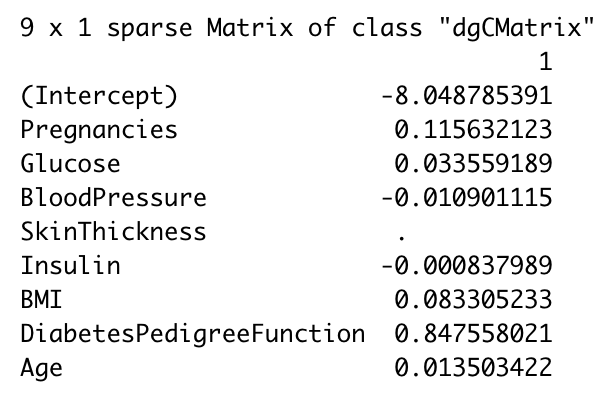
\includegraphics[width=0.6\textwidth]{img/pima-glmnet-output.png}
\end{center}
Compare this output to the results of models obtained through forward and backward selection methods, as well as to the full (unregularized) logistic regression model. What are the advantages and disadvantages of the regularization approach vs. wrappers and filters?
\end{question}

%%%%%%%%%%%%%%%%%%%%%%%%%%%%%%%%%%%%%%%%%%%%%%%%%%%%%%%%%%%%%%%%%%%%%%

